\section{绪论}

\subsection{动物实验}

\sy{动物实验}可如下分类:(\autoref{tab:动物实验的两种类型})

\begin{table}[htbp]
	\centering
	\begin{tabularx}{\textwidth}{|c|c|C|}
		\hline
		\textbf{实验类型} & \textbf{对象} & \textbf{特点} \\ \hline
		急性实验 & 活体标本或完整动物 & 条件人为控制,时间短,有损伤性 \\ \hline
		慢性试验 & 完整、清醒的动物 & 环境接近常态,时间长,因素多 \\ \hline
	\end{tabularx}
	\caption{动物实验的两种类型}
	\label{tab:动物实验的两种类型}
\end{table}

急性实验还可分为\sy{在体实验}和\sy{离体实验},区别就是实验材料是否在动物体内。

动物实验的\sy{3R原则}:\zhongdian{减少(Reduction)、替换(Replacement)、改进(Refinement)}	。

最容易引发可兴奋组织兴奋的电刺激波形是\zhongdian{矩形波(方波)},因为它是突变的。

\subsection{机体生理功能的调节}

包括\sy{神经调节}、\sy{体液调节}、\sy{自身调节}。

\zhongdian{自身调节}是某些细胞、组织、器官依靠自身特性感知内环境变化并作出改变的过程,\zhongdian{不需要神经支配或激素调控}。

\subsection{前馈控制系统}

与反馈控制不同,前馈控制是开环的。前馈控制是通过其它干扰对“控制中心”发挥作用的方式。

如冬泳前,未入水,体温还没降低,机体就通过感知空气的寒冷而提前产热,这就是前馈。而负反馈是,等到进入水中,体温降低才开始产热。

前馈具有预见性,但也可能造成浪费。

\section{细胞电活动}

细胞生物电是一些离子跨膜流动产生的,表现为一定的膜电位。机体内所有细胞都有静息电位,但只有神经细胞、肌细胞、部分腺细胞才有动作电位。并非所有活细胞都有稳定的静息电位(如有自律性的细胞)。

心电图、脑电图等是在器官水平上记录的生物电,是许多细胞电活动的总和。

\subsection{静息电位}

\subsubsection{静息电位的测定和概念}

参考电极置于接地的细胞外液中,使其保持零电位;测量电极是极细的玻璃微电极,测得细胞内为负电位。

这种内负外正的状态,就是静息电位。

\subsubsection{静息电位的产生}

静息电位的形成是各种离子跨膜移动的电驱动力(阻力)和浓度梯度(驱动力)达到平衡的结果。而离子跨膜移动最原始的浓度差则依靠各种离子泵,主要是钠钾泵来建立。

若细胞膜只对\ce{K+}有通透性,则由于细胞内\ce{K+}浓度高,胞外\ce{K+}浓度低,胞内\ce{K+}会向胞外扩散,这就是浓度差驱动的扩散。与此同时,带负电荷的有机离子因不能透过膜而留在胞内,这种负电荷对\ce{K+}的吸引将\ce{K+}限制在膜的外表面。这就产生了内负外正的电位差,即\ce{K+}扩散电位。

离子浓度差和跨膜电场这两个影响离子跨膜流动的驱动力的代数和称为离子的电-化学驱动力,其为0时,膜两侧的电位差便稳定下来。

可以使用能斯特方程计算某种离子的平衡电位(单位是\si{\V}):

\[E_X = \frac{RT}{nF} \ln \frac{c_\text{o}}{c_\text{i}}\]

在体温为\SI{37}{\degreeCelsius}时,该公式可简化为:(单位是\si{\mV})

\[E_X = \frac{61.5}{n} \lg \frac{c_\text{o}}{c_\text{i}}\]

事实上,在静息状态下,细胞膜对\ce{K+}的通透性是最大的,因为细胞膜上存在持续开放的非门控\ce{K+}通道,如神经细胞膜上的钾漏通道。而细胞膜对\ce{Na+}也有微弱的通透性,少量进入细胞的\ce{Na+}可以抵消一部分\ce{K+}产生的膜内负电位。

实验测得静息电位与\ce{K+}平衡电位十分接近,但是略低。这表明\ce{K+}对静息电位贡献最大,但静息电位是多种离子共同作用的结果。

钠钾泵的活动相当于将一个正电荷移出胞外,从而引起膜超极化,不过这种生电作用对静息电位的贡献不大。它还维持了细胞内外\ce{Na+}和\ce{K+}的浓度差。故钠钾泵活动越强,细胞内静息电位负值越大。

影响细胞膜静息电位的因素:
\begin{itemize}
	\item 细胞外液\ce{K+}、\ce{Na+}浓度;
	\item 膜对液\ce{K+}、\ce{Na+}的通透性;
	\item 钠泵活动水平。
\end{itemize}

\subsection{动作电位}

在静息电位基础上、细胞受到适当刺激后,膜电位发生的膜电位的迅速、可逆、可以向远距离传播的电位波动。有动作电位的细胞称为可兴奋细胞。

锋电位、后电位

动作电位的三个特点:
\begin{enumerate}
	\item 全或无
	\item 不衰减
	\item 脉冲式
\end{enumerate}

\subsubsection{动作电位的产生机制}

\subsubsection{动作电位的传导、传递}

郎飞氏结:髓鞘的空缺区域 密集的\ce{Na+}门控通道  跳跃式传导减少能量消耗、加快速度

缝隙连接(电突触)

兴奋性的变化 仅有绝对不应期和相对不应期

传导的一般特点:
\begin{description}
	\item[生理完整性]
\end{description}

神经干复合动作电位

\subsection{电紧张电位和局部电位}

\subsubsection{细胞膜和胞质的被动电学特征}

细胞膜和胞质作为一个静态的(无离子通道参与)的电学元件所表现出的性质,即被动电学特征,包括膜电容、膜电阻、轴向电阻。





\section{肌细胞和肌肉}












\section{血液}

\subsection{血液生理概述}

\subsubsection{血液的组成}

血液=血浆+血细胞。

\paragraph{血浆}

血浆包括水、电解质、有机物、气体。这些物质易透过膜,故血浆中的电解质含量与组织液中的基本相同。

\subparagraph{血浆蛋白}

血浆与组织液的最大区别就是血浆蛋白较多。

血浆蛋白可用盐析法分为球蛋白、白蛋白、纤维蛋白原三类。

三者的特点如下:

\begin{description}
	\item[含量] 白蛋白最多。
	\item[带电性] 白蛋白带负电,球蛋白带正电。
	\item[产生] 白蛋白和大多数球蛋白都来源于肝脏,仅$\upgamma$-球蛋白来源于浆细胞(效应B细胞)。肝病时白蛋白减少,$\upgamma$-球蛋白增多。
\end{description}

血浆蛋白的功能:

\begin{enumerate}
	\item 形成血浆胶体渗透压(尤其是白蛋白);
	\item 与激素可逆性结合,延长半衰期;
	\item 作为载体运输脂质、维生素、代谢废物;
	\item 参与凝血、抗凝、纤溶等过程;
	\item 免疫;
	\item 营养。
\end{enumerate}

\paragraph{血细胞}

血细胞包括红细胞、白细胞、血小板,红细胞最多,\zhongdian{白细胞最少}。

离心时,从上到下分为三层:血浆、白细胞和血小板、红细胞。

\sy{血细胞比容}是血细胞在血液中的体积占比。\zhongdian{新生儿最大},其次为男性。因为红细胞占绝对多数,故\zhongdian{血细胞比容可反映红细胞的相对浓度}。

\subsubsection{血液的理化特性}

\paragraph{比重}

血液的比重主要取决于红细胞数量;血浆的比重主要取决于血浆蛋白的含量;红细胞的比重取决于血红蛋白含量。

\paragraph{黏度}

温度不变时,全血的黏度取决于血细胞比容、血流切率;血浆的黏度取决于血浆蛋白含量。

血液黏度是形成血流阻力的因素之一。

\paragraph{渗透压}

\sy{范托夫定律}:\zhongdian{溶液渗透压的高低取决于溶质微粒数目的多少,与溶质的种类或大小无关。}

血浆渗透压包括晶体渗透压和胶体渗透压两部分,\zhongdian{晶体渗透压占主要}。而胶体渗透压中,由于\zhongdian{白蛋白分子量小,微粒数多,故是胶体渗透压的主要成分}。

血浆蛋白不易通过毛细血管壁,故血浆胶体渗透压虽小,但是在调节水平衡、维持正常血浆容量中发挥重要作用。血浆蛋白降低时,会发生组织水肿。

等渗溶液与等张溶液的区别:
\begin{itemize}
	\item 等渗溶液仅仅指的是渗透压与细胞内相等;
	\item 等张溶液还要求红细胞在溶液中不变形;
	\item 等渗溶液不一定等张,等张溶液一定等渗。
	\item 如0.9\%\ce{NaCl}是等张溶液,1.9\%尿素等渗而不等张。
\end{itemize}

\paragraph{pH}

正常血浆pH:7.35\textasciitilde7.45。

血浆pH的维持有赖于三个酸碱缓冲对:HCO$_{3}^{-}$/\ce{H2CO3}、蛋白质阴离子/蛋白质、HPO$_{4}^{2-}$/\ce{H3PO4},其中\zhongdian{HCO$_{3}^{-}$/\ce{H2CO3}最重要}。

\subsubsection{血液的免疫特性}

血液中包含免疫系统三部分的其二:免疫细胞、免疫分子(还有一个是免疫器官和组织)。血液中的血细胞、抗体、补体均是免疫系统的重要组成部分。

\paragraph{非特异性免疫}

非特异性免疫由遗传获得,又称固有免疫。

\begin{description}
	\item[固有免疫细胞] 吞噬细胞、树突状细胞(DC)、自然杀伤细胞(NK细胞)、自然杀伤T细胞、$\upgamma\updelta$T细胞、B1细胞等。
	\item[固有免疫分子] 补体。
\end{description}

\paragraph{特异性免疫}

特异性免疫是后天通过接触抗原物质或接受免疫效应因子获得的免疫,又称获得性免疫。获得性免疫分为细胞免疫和体液免疫两类。有关内容见高中教科书。

\begin{description}
	\item[获得性免疫细胞] B淋巴细胞、T淋巴细胞。
	\item[获得性免疫分子] 抗体。
\end{description}

\subsection{血细胞}

\subsubsection{血细胞的生成}

各类血细胞均起源于骨髓造血干细胞。造血就是各类造血细胞发育成熟的过程。造血过程分为:造血干细胞$\longrightarrow$造血祖细胞$\longrightarrow$形态可辨认的前体细胞这三个阶段。

\begin{description}
	\item[造血干细胞] 具有对称性和非对称性有丝分裂能力。通过对称性有丝分裂增殖,通过非对称性有丝分裂产生一个早期祖细胞和一个干细胞。
	\item[造血祖细胞] 仅进行对称性有丝分裂,边增殖边分化。体外培养时,可形成集落形成单位(CFU),分别有:红系集落形成单位(CFU-E)、粒-巨噬细胞集落形成单位(CFU-GM)、巨核系集落形成单位(CFU-MK)、淋巴系集落形成单位(CFU-L)。

	早期造血祖细胞还具有多向分化能力,如髓系多向造血祖细胞(CFU-GEMM)、CFU-L;晚期造血祖细胞定向分化为各种前体细胞。早期和晚期红系祖细胞分别形成很大的红系爆式集落形成单位(BFU-E)和较小的CFU-E。
	\item[前体细胞] 已经发育为形态可辨的细胞,进一步分化成熟即成为成熟血细胞。
\end{description}

造血龛(造血微环境)是造血干细胞定居并最终分化为成熟血细胞的场所。包括:
\begin{itemize}
	\item 造血器官中的基质细胞;
	\item 基质细胞分泌的细胞外基质;
	\item 造血调节因子;
	\item 进入造血器官的神经和血管。
\end{itemize}

基质细胞包括骨髓中的各种细胞,能产生细胞因子,调控造血干细胞的增殖和分化。若静脉输入造血干细胞,其能很快归巢至骨髓,与其表达的黏附蛋白有关。

\subsubsection{红细胞}

\paragraph{数量和形态}

红细胞是血液中数量最多的细胞。儿童少于成年人,新生儿多于成年人,高原居民多于平原居民,妊娠后期因血浆增多而红细胞比容相对减少。

正常的哺乳动物成熟红细胞无核和其他细胞器,呈两面凹的圆盘状。红细胞维持这种形状需要耗能。糖酵解是成熟红细胞唯一产能方式。

\paragraph{生理特征}

\begin{description}
	\item[可塑变形性] 是红细胞在外力作用下变形的特性。红细胞的形状使其拥有大的比表面积,对该性状贡献最大。可塑变形性使得红细胞可以穿过毛细血管壁。
	\item[悬浮稳定性] 是红细胞在血浆中缓慢下沉的特性。红细胞有大比表面积$\rightarrow$较大摩擦力。红细胞发生叠连时下沉变快。红细胞表面带负电荷相斥,故带正电物质(纤维蛋白原、球蛋白、胆固醇)可加速叠连,带负电荷物质(白蛋白、卵磷脂)可减慢叠连。
	\item[渗透脆性] 是在低渗盐溶液中发生涨破的特性。红细胞可以抵抗一定的低渗环境,而且同一个体的不同红细胞抵抗能力不同。衰老红细胞的脆性高,新生红细胞的脆性低。
\end{description}

\paragraph{功能}

红细胞内的血红蛋白以氧合血红蛋白运输\ce{O2},以氨基甲酰血红蛋白运输\ce{CO2}。

\paragraph{红细胞生成}

骨髓是产生红细胞的唯一场所。红细胞的产生过程如下:

造血干细胞$\longrightarrow$红系造血祖细胞$\longrightarrow$原红细胞$\xrightarrow{\text{多次有丝分裂}}$早幼红细胞$\xrightarrow{\text{多次有丝分裂}}$中幼红细胞$\xrightarrow{\text{多次有丝分裂}}$晚幼红细胞$\xrightarrow{\text{排出核}}$网织红细胞$\xrightarrow[\text{血液中}]{\text{自噬清除细胞器}}$成熟红细胞

晚幼红细胞通过不对称胞质分裂排出细胞核。

网织红细胞存在时间较短,故可通过血液中网织红细胞计数来判断骨髓造血功能盛衰。

\subparagraph{生成红细胞所需物质}

\begin{itemize}
	\item 主要:蛋白质、铁、叶酸、维生素B$_{12}$;
	\item 次要:维生素B$_{6}$、B$_{2}$、C、E,氨基酸,微量元素。
\end{itemize}

\begin{description}
	\item[蛋白质] 红细胞可优先利用体内的氨基酸来合成血红蛋白,较少出现因蛋白质缺乏而导致的贫血。
	\item[铁] 衰老红细胞被巨噬细胞吞噬后,释放的铁可再利用。人每天只需补充很少量的铁以弥补排泄损失。血液中的铁与转铁蛋白结合而被运送到幼红细胞。缺铁影响血红蛋白合成,导致缺铁性贫血。
	\item[叶酸和维生素B$_{12}$] 重要辅酶。维生素B$_{12}$参与叶酸在胞内的转化,叶酸参与DNA合成。缺二者其一都会导致核发育滞后于质,造成巨幼细胞性贫血。

	维生素B$_{12}$的吸收需要内因子,由胃黏膜壁层产生,二者结合,然后在回肠被受体介导内吞。

	维生素B$_{12}$储量多,用量少,消耗慢;叶酸储量更大,但消耗更多,消耗快。
\end{description}

\paragraph{红细胞生成的调节}

主要是对红系造血祖细胞的调控,早期和晚期祖细胞的受体不同,调节物质也就不同。

\begin{description}
	\item[BFU-E的刺激物] 干细胞因子(SCF)、白介素-3(IL-3)、粒-巨噬细胞集落刺激因子(GM-CSF)刺激其发育为CFU-E。
	\item[BFU-E的抑制物] TGF-$\upbeta$、干扰素$\upgamma$、肿瘤坏死因子。
	\item[CFU-E的刺激物] 促红细胞生成素(EPO)
\end{description}

可以抑制BFU-E增殖。


下面介绍EPO和性激素对红细胞生成的影响。

\subparagraph{促红细胞生成素(EPO)}

EPO的促红细胞生成作用:

\begin{itemize}
	\item 抑制CFU-E凋亡,CFU-E完全依赖EPO而存活。
	\item 激活血红蛋白等特异基因的表达。
	\item 促进网织红细胞的生成和释放。
\end{itemize}

正常情况下血浆中存在少量EPO,维持红细胞产生。血浆EPO的水平与血液血红蛋白浓度负相关。EPO水平与红细胞数存在负反馈。

除了CFU-E,脑、心、血管内皮也存在EPO受体\footnote{EPO受体都是I型细胞因子受体,信号通路为JAK-STAT。},也产生抗凋亡效应。

主要由皮质肾单位的肾小管周围的间质细胞(主要是成纤维细胞)产生EPO。双肾严重破坏者发生肾性贫血。肾内没有EPO的储存。肾外组织(如肝)可产生少量EPO。

缺氧可诱导EPO产生。路径如下:

低氧$\longrightarrow$转录因子HIF-1活性$\uparrow$$\longrightarrow$与\textit{EPO}基因增强子结合$\longrightarrow$EPO表达$\uparrow$

甲状腺激素、肾上腺皮质激素、生长激素可改变组织对氧的需求,从而提高EPO生成。

\subparagraph{性激素}

\begin{itemize}
	\item 雄激素刺激EPO产生、刺激BFU-E和CFU-E、促进血红蛋白合成;
	\item 雌激素可以降低红细胞对EPO的反应,抑制红细胞生成。
\end{itemize}

\paragraph{红细胞的破坏}

正常人红细胞寿命约120天。红细胞衰老后有两种破坏方式:

\begin{description}
	\item[血管外破坏] 红细胞破坏的主要方式。衰老红细胞因为变形能力减退,而容易滞留在肝、脾、骨髓中被巨噬细胞吞噬。巨噬细胞将血红蛋白消化:铁和氨基酸重新利用,胆红素进入胆汁排出体外。
	\item[血管内破坏] 少数是这样。红细胞因为机械冲击而破损,释放出的血红蛋白被\sy{触珠蛋白}结合$\rightarrow$被肝脏摄取。若红细胞大量破坏,超出触珠蛋白结合上限,就会出现血红蛋白尿。
\end{description}

\subsubsection{白细胞}


\paragraph{分类和数量}

白细胞分为中性粒细胞、嗜酸性粒细胞、嗜碱性粒细胞、单核细胞、淋巴细胞五类。前三类统称为粒细胞。

血液中最多的是中性粒细胞,其次是淋巴细胞。血液中可以没有嗜碱性粒细胞。

白细胞的数目波动:

\begin{itemize}
	\item 新生儿白细胞较多;
	\item 下午白细胞多于早上;
	\item 进食、疼痛、情绪激动、剧烈运动、妊娠末期和分娩时增多。
\end{itemize}

\paragraph{生理功能}

白细胞主要通过两种方式来抵御外源性病原体的入侵:
\begin{enumerate}
	\item 吞噬作用;
	\item 形成抗体或和致敏淋巴细胞。
\end{enumerate}

白细胞发生吞噬作用的过程如下:

\begin{description}
	\item[血细胞渗出] 除了淋巴细胞,所有白细胞都可以发生此过程,即白细胞做变形运动穿过毛细血管壁进入组织之间的过程。
	\item[趋化运动] 白细胞具有趋化性,可游走到炎症部位吞噬异物。趋化因子包括:细胞降解产物、抗原-抗体复合物、补体活化产物、细菌毒素、细菌等。
\end{description}

白细胞自己还可分泌白介素、干扰素、肿瘤坏死因子、集落刺激因子等细胞因子参与炎症和免疫反应。

白细胞的主要功能见\autoref{tab:白细胞的功能}。

\begin{table}[htbp]
	\centering
	\begin{tabularx}{\textwidth}{|C|c|c|c|}
		\hline
		\textbf{白细胞} & \textbf{形态特点} & \textbf{功能} & \textbf{特性} \\ \hline
		中性粒细胞 & \begin{tabular}[c]{@{}c@{}}核分叶,\\ 质中存在颗粒\end{tabular} & \begin{tabular}[c]{@{}c@{}}主要的吞噬细胞,\\ 非氧/依氧杀菌\end{tabular} & 循环池与边缘池 \\ \hline
		嗜碱性粒细胞 & 较大碱性染色颗粒 & 过敏反应 & 释放肝素、白三烯 \\ \hline
		嗜酸性粒细胞 & 含带正电荷的蛋白 & 抗过敏、蠕虫幼体 & \begin{tabular}[c]{@{}c@{}}糖皮质激素\\ 负相关的数量波动\end{tabular} \\ \hline
		单核细胞 & 巨噬细胞体积大 & \begin{tabular}[c]{@{}c@{}}MP超强吞噬能力,\\ DC抗原呈递\end{tabular} & 进入组织才成熟 \\ \hline
		淋巴细胞 & --- & \begin{tabular}[c]{@{}c@{}}NK固有免疫,\\ T、B特异性免疫\end{tabular} & 免疫应答的核心 \\ \hline
	\end{tabularx}
	\caption{白细胞的功能}
	\label{tab:白细胞的功能}
\end{table}

非氧杀菌和依氧杀菌:

\begin{description}
	\item[非氧杀菌] 通过水解酶、乳铁蛋白、杀菌通透性增加蛋白;
	\item[依氧杀菌] 产生大量活性氧基团。
\end{description}
\paragraph{白细胞生成的调节}

机体炎症反应时,促进中性粒细胞、单核细胞生成。

单核细胞只有进入组织中,才会发育成巨噬细胞或者树突状细胞。

\begin{itemize}
	\item 促进白细胞生成:GM-CSF、G-CSF、M-CSF;
	\item 抑制白细胞生成:乳铁蛋白、TGF-$\upbeta$。
\end{itemize}

\paragraph{白细胞的破坏}

白细胞在血液中停留的时间较短,进入组织发挥作用。\zhongdian{中性粒细胞在吞噬过量细菌后,便会发生自我溶解},残骸与细菌碎片形成\sy{脓液}。

\subsubsection{血小板}

\paragraph{血小板的数量和功能}

血小板无核,受刺激时可伸出伪足。内含$\upalpha$-颗粒、致密体。膜上有多种糖蛋白,作受体。

存在昼夜波动,午后比清晨多。静脉血中比毛细血管中多。

血小板有助于维持血管壁的完整性。

\paragraph{血小板的生理特性}

\begin{description}
	\item[黏附] 血管内皮细胞破损时,暴露出下方的胶原,vWF与胶原结合,vWF发生变构,使血小板与vWF结合。vWF发挥了桥梁作用。
	\item[释放] 血小板受刺激后排出储存在致密体、$\upalpha$-颗粒、溶酶体内的物质。

	血栓烷A$_{2}$(TXA$_{2}$)很特殊,它在血小板内没有储存,从膜磷脂经过环氧合酶和血栓烷合成酶的作用下合成。
	\item[聚集] 血小板之间相互黏着。需要纤维蛋白原(不是纤维蛋白)、\ce{Ca^{2+}}、膜上GP IIb/IIIa参与。
	\item[收缩] 类似肌细胞的收缩。
	\item[吸附] 血小板表面吸附多种凝血因子,利于凝血。
\end{description}

\paragraph{血小板的生成调节}

血小板来源于巨核细胞胞质裂解产物。

血小板生成素(TPO)是重要的调节因子,主要由肝合成,少量由肾合成\footnote{这与EPO的合成恰好相反。}。TPO可促进巨核系祖细胞的增殖。TPO对造血干细胞的存活、增殖、分化也有重要作用。

\paragraph{血小板的破坏}

血小板在衰老或发挥生理功能时被破坏。衰老的血小板在脾、肝、肺部被破坏。

\subsection{生理性止血}

\subsubsection{止血的基本过程}

止血的基本过程包括三个过程:

\begin{description}
	\item[血管收缩] 引发因素:反射性收缩、肌源性收缩、血小板释放5-HT、TXA$_{2}$等缩血管物质。
	\item[血小板止血栓形成] 损伤血管内皮下胶原暴露,使血小板黏附。()
	\item[血液凝固] 此为二期止血,启动凝血系统,生成纤维蛋白。
\end{description}


\subsubsection{二期止血的详细机制}

纤维蛋白是目前发现弹性最好的蛋白质,使得血凝块有良好的弹性。

\paragraph{凝血因子}

凝血因子共14种,罗马数字编号的有12种,从FI到FXIII(少了FVI,其实是FVa)。

几个特殊的凝血因子:

\begin{itemize}
	\item 丝氨酸蛋白酶:2、7、9、10、11、12;
	\item 依赖维生素K:2、7、9、10;
	\item 不在肝合成:3、5、(13)\footnote{凝血因子XIII在肝细胞和血小板都可以合成。}
	\item 与血友病有关:8A 9B 11C。
\end{itemize}
\section{血液循环}

\subsection{心脏的泵血功能}

\subsubsection{心动周期}

\subsubsection{影响心输出量的因素}

\subsubsection{评价心脏泵血功能的指标}

\subsubsection{心音}

心音是心肌收缩、瓣膜启闭、血流撞击或湍流而产生的声音。心音的听诊特点:

\begin{itemize}
	\item 一般只可以听到第一、第二心音;
	\item 部分健康儿童和青年人可听到第三心音;
	\item \zhongdian{健康人听不到第四心音,若心房收缩强烈或左心室顺应性降低则可以听到。}
\end{itemize}

四种心音的产生见\autoref{tab:四个心音}。

\begin{table}[htbp]
	\centering
	\begin{tabularx}{\textwidth}{|c|C|C|}
		\hline
		心音 & 成因 & 出现时机 \\ \hline
		第一心音 & 房室瓣关闭 & 心室收缩开始 \\ \hline
		第二心音 & 动脉瓣关闭 & 心室舒张期开始 \\ \hline
		第三心音 & 心室壁伸展、血流减速 & 快速充盈期末 \\ \hline
		第四心音 & 心房收缩 & 心室舒张晚期 \\ \hline
	\end{tabularx}
	\caption{四个心音}
	\label{tab:四个心音}
\end{table}

\subsection{心脏的电生理}

心肌细胞具有兴奋性、传导性、自律性、收缩性。

心肌细胞可分为\autoref{fig:心肌细胞的分类}。

\begin{figure}[htbp]
	\centering
	\begin{forest}
		forest scheme
		[心肌细胞
			[快反应工作细胞(收缩)
				[心房肌细胞]
				[心室肌细胞]]
			[慢反应自律细胞
				[窦房结]
				[房室结]]
			[快反应自律细胞
				[浦肯野细胞]]]
	\end{forest}
	\caption{心肌细胞的分类}
	\label{fig:心肌细胞的分类}
\end{figure}

\subsection{心肌细胞的跨膜电位}

不同心肌细胞的跨膜电位变化不同。

\subsubsection{工作细胞}

\paragraph{静息电位}

静息电位与一般的神经元或骨骼肌相似。

成分:

\begin{description}
	\item[内向整流\ce{K+}通道(I$_{\text{K1}}$)] \sy{离子通道的整流特性}指的是,离子通道在不同膜电位下,对离子通透性产生变化。I$_{\text{K1}}$对\ce{K+}的通透性随去极化而降低。
	\item[\ce{Na+}-\ce{K+}泵的生电作用]
	\item[\ce{Na+}的部分内流]
\end{description}

\paragraph{心室肌细胞动作电位}

心室肌细胞动作电位分为5个阶段:

\begin{itemize}
	\item 0期:自动去极化期;
	\item 1期:快速复极化初期;
	\item 2期:平台期;
	\item 3期:快速复极化末期;
	\item 4期:完全复极化期。
\end{itemize}

动作电位时程(APD):0期自动去极化开始到3期复极化完毕这段时间的长度。心室肌细胞的APD为200\textasciitilde\SI{300}{\ms}。

\begin{table}[htbp]
	\centering
	\begin{tabularx}{\textwidth}{|c|C|C|c|c|}
		\hline
		时期 & 内向电流 & 外向电流 & 膜电位 & 时程 \\ \hline
		0期 & I$_{\text{Na}}$$\uparrow$ & I$_{\text{K1}}$$\downarrow$ & -90\textasciitilde\SI{+30}{\mV} & \SI{1.5}{\ms} \\ \hline
		1期 &  &  &  &  \\ \hline
		2期 &  &  &  &  \\ \hline
		3期 &  &  &  &  \\ \hline
		4期 &  &  &  &  \\ \hline
	\end{tabularx}
	\caption{心室肌细胞动作电位}
	\label{tab:心室肌细胞动作电位}
\end{table}

\subsubsection{心电图}

\paragraph{心电图的原理}

\paragraph{心电图的绘制}

记录心电图时,电极的放置位置、与心电图机连接的线路称为心电图导联。不同导联记录到的心电图波形不同,但是成分相同,都包含P波、QRS波群、T波、有时可见U波。

\autoref{tab:心电图特征}总结了II型导联的心电图特征。

\begin{table}[htbp]
	\centering
	\begin{tabularx}{\textwidth}{|c|c|c|C|}
		\hline
		\textbf{时期} & \textbf{波形/时程} & \textbf{生理过程} & \textbf{异常状况} \\ \hline
		P波 & 小而圆钝 & 心房去极化 & \begin{tabular}[c]{@{}c@{}}消失:房颤\\ 增幅:右心房肥大;\\延长或双峰:左心房肥大;\end{tabular} \\ \hline
		PQ间期 & P始-QRS始 & 房室传导时间 & 延长:房室传导阻滞 \\ \hline
		QRS波群 & 下--上--下 & 心室去极化 & \begin{tabular}[c]{@{}c@{}}增宽:心室传导阻滞;\\ 增幅:心肌肥厚\end{tabular} \\ \hline
		QT间期 & QRS始-T终 & 心室去极化到复极化 & 时程变化:离子通道 \\ \hline
		ST段 & QRS终-T始 & 心室平台期 & 升或降:心肌损伤 \\ \hline
		T波 & 低幅,上 & 心室复极化 & T波改变 \\ \hline
		U波 & 低而宽 & 不明 & 低血钾 \\ \hline
	\end{tabularx}
	\caption{心电图特征}
	\label{tab:心电图特征}
\end{table}

\subsection{血管生理}

体循环占血流量的大部分,体循环中静脉血占比最大。

\subsubsection{各类血管的功能特点}

\paragraph{血管壁的结构}

血管系统中。动脉、毛细血管、静脉依次串联。动脉和静脉管壁可分为如\autoref{fig:血管壁的组成}所示的结构。

\begin{figure}[htbp]
	\centering
	\begin{forest}
		forest scheme
		[血管壁
		[内膜
		[内皮细胞
		[通透性屏障]
		[为血流提供光滑表面]
		[内分泌]]
		[内皮下层]]
		[中膜
		[血管平滑肌
		:调节血流量]
		[弹性纤维
		:使动脉扩张或回缩]
		[胶原纤维]]
		[外膜
		[疏松结缔组织
		:含间质细胞、微血管]]]
	\end{forest}
	\caption{血管壁的组成}
	\label{fig:血管壁的组成}
\end{figure}

\paragraph{血管的功能性分类}

\begin{description}
	\item[弹性贮器血管]
	\item[分配血管]
	\item[毛细血管前阻力血管]
	\item[毛细血管前括约肌]
	\item[毛细血管] 又称交换血管
	\item[毛细血管后阻力血管]
	\item[容量血管] 即静脉系统
	\item[短路血管] 小动脉和小静脉不经毛细血管直接相连。
\end{description}

\paragraph{血管的内分泌功能}

\begin{description}
	\item[血管内皮细胞] 合成舒血管(NO、\ce{H2S}、前列环素)和缩血管(内皮素、TXA$_{2}$)物质。
	\item[血管平滑肌细胞] 合成分泌肾素、血管紧张素。
	\item[其他细胞] 如成纤维细胞和脂肪细胞等,除了保护、支持、营养作用以外,还可分泌血管紧张素等物质。
\end{description}

\subsubsection{血流动力学}

\paragraph{血流的物理参数}

血流量指的是单位时间内流过的血液体积;血流速度指的是血液中一个质点的线速度。

\subparagraph{泊肃叶定律}

液体流量\[Q=\frac{\uppi\upDelta Pr^4}{8\upeta L}\]

血管直径是影响血流量的主要因素。

\subsubsection{动脉}

\autoref{tab:影响动脉血压的因素}

\begin{table}[htbp]
	\centering
	\begin{tabularx}{\textwidth}{|cC|C|C|C|}
		\hline
		\multicolumn{2}{|c|}{因素} & 收缩压 & 舒张压 & 脉压 \\ \hline
		\multicolumn{1}{|c|}{\multirow{2}{*}{每搏输出量}} & $\uparrow$ & $\uparrow$$\uparrow$ & $\uparrow$ & $\uparrow$ \\ \cline{2-5}
		\multicolumn{1}{|c|}{} & $\downarrow$ & $\downarrow$$\downarrow$ & $\downarrow$ & $\downarrow$ \\ \hline
		\multicolumn{1}{|c|}{\multirow{2}{*}{心率}} & $\uparrow$ & $\uparrow$ & $\uparrow$$\uparrow$ & $\downarrow$ \\ \cline{2-5}
		\multicolumn{1}{|c|}{} & $\downarrow$ & $\downarrow$ & $\downarrow$$\downarrow$ & $\uparrow$ \\ \hline
		\multicolumn{1}{|c|}{\multirow{2}{*}{外周阻力}} & $\uparrow$ & $\uparrow$ & $\uparrow$$\uparrow$ & $\downarrow$ \\ \cline{2-5}
		\multicolumn{1}{|c|}{} & $\downarrow$ & $\downarrow$ & $\downarrow$$\downarrow$ & $\uparrow$ \\ \hline
		\multicolumn{1}{|c|}{动脉弹性} & $\downarrow$ & $\uparrow$ & $\downarrow$ & $\uparrow$ \\ \hline
	\end{tabularx}
	\caption{影响动脉血压的因素}
	\label{tab:影响动脉血压的因素}
\end{table}

除此之外,循环血量和血管容量的匹配程度也会影响动脉血压。如大失血时,血压降低。

\section{呼吸}

在人和高等动物中,呼吸分为三个环节:(\autoref{fig:3steps_breath})
\begin{figure}[htbp]
	\centering
	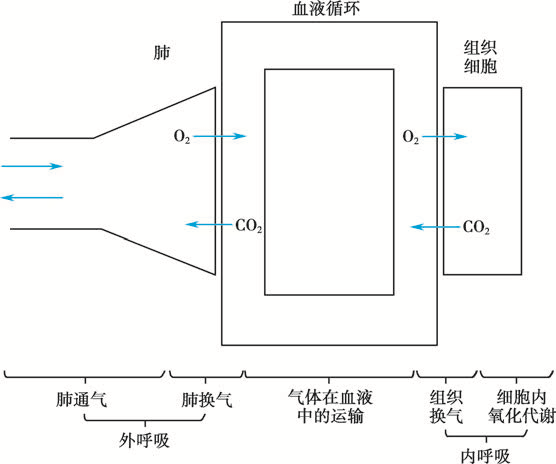
\includegraphics[width=0.7\linewidth]{Pics/呼吸的三个环节}
	\caption{呼吸的三个环节}
	\label{fig:3steps_breath}
\end{figure}

\begin{description}
	\item[外呼吸] 肺毛细血管中血液与外界环境气体交换的过程,包括:肺通气、肺换气;
	\item[气体运输] \ce{O2}和\ce{CO2}在血液中的运输;
	\item[内呼吸] 组织细胞与组织毛细血管之间的气体交换(组织换气)、组织细胞内氧化代谢。
\end{description}

\subsection{肺通气}

实现肺通气的器官和过程有:
\begin{description}
	\item[呼吸道] 是气体进出的通道,从气管到肺泡共分23级。
	\item[肺泡] 临近的肺泡通过小孔相连(肺泡相互依存),增加结构稳定性,防塌陷。
	\item[胸膜腔] 连接肺和胸廓,肺表面和胸廓内壁之间的腔隙,无气体、仅有很薄一层浆液。浆液形成胸膜腔内负压、润滑;
	\item[膈和胸廓] 其上的胸壁肌产生呼吸动力。
\end{description}

\subsubsection{肺通气的动力}

\begin{itemize}
	\item 直接动力:肺泡气与外界大气之间的压力差;
	\item 原动力:呼吸肌的收缩与舒张引起的节律性呼吸运动。
\end{itemize}

呼吸运动按参与的肌肉分为胸式呼吸和腹式呼吸,按呼吸的用力程度分为平静呼吸和用力呼吸。\zhongdian{在用力呼吸时,肋间外肌参与主动呼气过程。}(\autoref{tab:breathing_patterns})

\begin{table}[htbp]
	\centering
	\begin{tabularx}{\textwidth}{|c|c|c|C|}
		\hline
		呼吸形式 & 肌肉 & 起伏 & 人群 \\ \hline
		胸式呼吸 & 肋间外肌 & 胸部 & 膈肌运动受限者:孕妇、胀气者 \\ \hline
		腹式呼吸 & 膈肌 & 腹部 & 胸廓运动受限者:胸腔积液者;婴儿\footnotemark \\ \hline
	\end{tabularx}

	\mbox{}\vspace{1em}

	\begin{tabularx}{\textwidth}{|c|C|C|c|c|}
		\hline
		呼吸形式 & 时机 & 肌肉 & 吸气 & 呼气 \\ \hline
		平静呼吸 & 安静状态 & 少 & \multirow{2}{*}{主动} & 被动 \\ \cline{1-3} \cline{5-5}
		用力呼吸 & 劳动或呼吸不畅 & 多(包括呼气肌) &  & 主动 \\ \hline
	\end{tabularx}

	\caption{呼吸形式}
	\label{tab:breathing_patterns}
\end{table}
\footnotetext{婴儿采用腹式呼吸的原因是婴儿的肋骨运动不易扩大胸腔容量。}

肺内压是肺泡内气体的压力。肺内压与大气压的压力差使气体出入肺部。人工呼吸就是人工地建立肺内压与大气压的压力差。

胸膜腔内压简称胸内压,可用测量食管内压的变化来间接反映胸内压的变化。胸膜腔内压在平静呼吸时始终低于大气压,即始终为负压;但是在用力呼气时,可大大高于(\SI{110}{mmHg})大气压。

胸膜腔内压的形成因素:
\begin{itemize}
	\item 胸廓的自然容积大于肺的自然容积,胸膜腔受胸廓的外向回位力和肺的内向回位力作用。随着个体发育,负压逐渐增大(变得更负);
	\item 肺内压使肺泡扩张,肺回缩压使肺泡缩小。$\text{胸内压}=\text{肺内压}-\text{肺回缩压}$,气流停止时,即$\text{胸内压}=\text{大气压}-\text{肺回缩压}$,可见肺回缩压主要决定了胸膜腔内压;
\end{itemize}

胸膜腔负压的意义:
\begin{itemize}
	\item 扩张胸导管、腔静脉,有利于淋巴液、静脉血的回流;
	\item 使肺保持扩张。
\end{itemize}

胸膜腔若破裂与外界大气相通,就形成气胸,导致肺不张,会危及生命。

\subsubsection{肺通气的阻力}

肺通气的阻力分为弹性阻力和非弹性阻力。弹性阻力在气流静止的情况下仍然存在,故亦称静态阻力;非弹性阻力仅在气流流动的情况下存在,故亦称动态阻力。

\paragraph{弹性阻力}

\subparagraph{顺应性}

顺应性是指弹性组织在外力作用下发生变形的难易程度。顺应性可用单位大小跨壁压的变化($\upDelta P$)所引起的容积变化($\upDelta V$)来表示:\[C=\frac{\upDelta V}{\upDelta P}\]
顺应性与弹性阻力是倒数关系。

肺顺应性的概念与此相同。在呼吸道无气流状态下可测得肺的静态顺应性。此时跨肺压(即肺的跨壁压$\upDelta P$)就是胸膜腔内压与大气压之差。绘制不同跨肺压下肺的体积的函数图象可根据斜率直观判断此处顺应性的大小。

肺顺应性的数值还受到肺总量的影响,肺总量大的人与肺总量小的人,吸入相同体积的气体,所产生的跨壁压是不同的。为了排除肺总量的影响,将肺顺应性除以肺总量,得到比顺应性。由于平静呼吸是从功能余气量开始的,所以肺的比顺应性还可以用顺应性除以功能余气量:\[\text{比顺应性}=\frac{\text{顺应性}}{\text{功能余气量}}\]

\subparagraph{肺弹性阻力$C_{\text{L}}$}

肺弹性阻力的来源有二:肺的弹性成分、肺泡表面张力。

肺的弹性成分即肺自身的纤维等结构。

肺泡表面张力源于肺泡内液-气表面能使液体表面积缩小的力。在肺的压力-容积曲线中,充入空气时肺萎陷和扩张的曲线并不重合,称为滞后现象。

从曲线中还可以看出,肺的弹性阻力主要来源于肺泡表面张力,因为充入生理盐水时,无肺泡表面张力,图象就更陡峭,表明此时弹性阻力更小。

\begin{figure}[htbp]
	\centering
	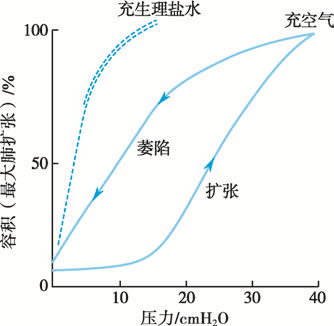
\includegraphics[width=0.3\linewidth]{Pics/肺的压力-容积曲线}
	\caption{肺的压力-容积曲线}
	\label{fig:p-v_curve_lung}
\end{figure}

\subparagraph{肺表面活性物质}

肺泡内表面(与外界空气接触的那一侧)具有肺表面活性物质(PS)。这是由肺泡II型上皮细胞合成和分泌的脂质与蛋白质的混合物。

\begin{figure}
	\centering
	\begin{forest}
		forest scheme
		[肺表面活性物质
			[脂质(90\%)
				[\zhongdian{二棕榈酰卵磷脂(DPPC)(大于60\%)}]
				[其他脂质]]
			[表面活性物质结合蛋白(SP)(10\%)]]
	\end{forest}
	\caption{肺表面活性物质的组成}
	\label{fig:constitution_lung_ps}
\end{figure}

DPPC是两亲分子,有亲水的头部和疏水的尾部,以疏水的一端朝向肺泡腔,可以降低表面张力。

肺表面活性物质的生理意义:
\begin{itemize}
	\item 减小吸气阻力;
	\item 维持不同大小肺泡的稳定性;
		\begin{itemize}
			\item 肺泡缩小时,PS分布的密度增大,减小表面张力防塌陷;
			\item 肺泡扩张时,PS分布的密度减小,增大表面张力防破裂。
		\end{itemize}
	\item 防止肺水肿,减小了表面张力对血管和组织液中水分的抽吸作用。
\end{itemize}

早产儿可能因肺泡II型上皮细胞未成熟,缺少PS,引发新生儿呼吸窘迫综合征。

\paragraph{胸廓弹性阻力$C_{\text{chw}}$}

各情况如\autoref{tab:cchw_cases}所示。

\begin{table}[htbp]
	\centering
	\begin{tabularx}{\textwidth}{|C|C|C|C|C|}
		\hline
		容量百分比\footnotemark & 胸廓状态 & 呼吸状态 & 吸气 & 呼气 \\ \hline
		$<67\%$ & 压缩 & 呼气 & 动力 & 阻力 \\ \hline
		$=67\%$ & 自然状态 & 平静吸气末 & 无 & 无 \\ \hline
		$>67\%$ & 扩张 & 深吸气 & 阻力 & 动力 \\ \hline
	\end{tabularx}
	\caption{胸廓弹性阻力分类讨论}
	\label{tab:cchw_cases}
\end{table}
\footnotetext{指的是在胸廓牵引下,肺的容量占肺总量的百分比。}

肺和胸廓呈“串联”关系,所以总弹性阻力是二者之和,也就是二者顺应性的倒数之和。

\subsubsection{非弹性阻力}

非弹性阻力包括惯性阻力、粘滞阻力、气道阻力。其中,气道阻力占大部分,下面仅讨论气道阻力。

气道阻力可用下面式子表示:\[\text{气道阻力}=\frac{\text{大气压与肺内压之差}}{\text{单位时间内气体流量}}\]

其余内容和通气阻力的总结见\autoref{tab:friction_lung}。

\begin{table}[htbp]
	\centering
	\begin{NiceTabularX}{\textwidth}{cccX}[hvlines]
		\Block[c]{1-2}{阻力类型} &  & 阻力来源 & \Block[c]{1-1}{具体影响}\\
		\Block[v-center]{3-1}{弹性阻力} & \Block[v-center]{2-1}{胸廓阻力} & 胸廓的弹性物质 & 见\autoref{tab:cchw_cases}\\
		&  & 肺的弹性物质 & 次要 \\
		& 肺阻力 & 肺泡表面张力 & 主要 \\
		\Block[v-center]{9-1}{非弹性阻力} & \Block[v-center]{7-1}{气道阻力} & \Block[v-center]{5-1}{气道口径} & 跨壁压\\
		&  &  & 肺实质的牵引 \\
		&  &  & 交感兴奋增大口径、副交感兴奋减小口径 \\
		&  &  & 舒张气管:儿茶酚胺、PGE$_2$ \\
		&  &  & 收缩气管:PGF$_{2\upalpha}$、组胺、白三烯、高\ce{CO2} \\
		&  & 气流速度 & 速度越快,阻力越大\\
		&  & 气流形式 & 层流阻力小,湍流阻力大\\
		& 惯性阻力 & \Block[v-center]{2-2}{平静呼吸时几乎不起作用} & \\
		& 粘滞阻力 &  &
	\end{NiceTabularX}
	\caption{肺通气的阻力}
	\label{tab:friction_lung}
\end{table}

\section{消化和吸收}

消化分为物理性消化(磨碎、混匀食物)和化学性消化(涉及酶解)。消化后的营养成分透过消化道黏膜进入血液或淋巴,称为吸收。

\subsection{消化概述}

消化系统由消化道和消化腺构成。其中,消化道不仅受交感和副交感神经支配,自身还有一套肠神经系统。

\subsubsection{消化道平滑肌}

消化道平滑肌具有如下性质:

\begin{itemize}
	\item 兴奋性较低,收缩缓慢;\item 自律性;\item 紧张性,常常保持在轻微收缩状态;\item 伸展性,可容纳大量食物;\item 刺激的选择性,对电刺激不敏感而对机械刺激、温度、化学物质敏感。
\end{itemize}

电生理方面,消化道平滑肌具有静息电位、慢波电位、动作电位三种形式。

\begin{description}
	\item[静息电位] (绝对值)较低,存在波动。
	\item[慢波电位] 自发产生周期性的轻度去极化和复极化,频率较慢。慢波又称为基本电节律(BER),具体频率因部位而异。慢波起源于消化道纵肌和环肌之间的Cajal间质细胞(ICC),有缝隙连接。
	
	慢波去极化到达机械阈时,产生小幅度收缩;到达电阈时,产生动作电位。
	\item[动作电位] 在慢波去极化基础上发生,收缩幅度与动作电位频率正相关。
\end{description}

\subsubsection{消化腺的分泌功能}

消化腺分泌消化液。消化液主要成分:水、例子、消化酶、抗体、黏液等。

功能:

\begin{itemize}
	\item 稀释食物,降低食物渗透压;
	\item 提供适宜pH,以便消化酶发挥作用;
	\item 消化酶水解食物;
	\item 抗体、黏液、水可保护黏膜。
\end{itemize}


\subsubsection{消化道的神经支配}

\paragraph{外来神经}

交感神经节后纤维释放NE,一般抑制胃肠运动和分泌;副交感神经大部分释放Ach,激活M受体,促进运动和分泌,抑制括约肌,少数肽能神经纤维释放血管活性肠肽、P物质、脑啡肽、生长抑素等。

\paragraph{内在神经丛}

大部分消化道管壁内具有两层神经结构,统称\sy{肠神经系统}(ENS)分别是\sy{黏膜下神经丛}和\sy{肌间神经丛}。肠神经系统构成一个\zhongdian{相对独立的、完整的}整合系统。

外来神经对内在神经丛具有调控作用,但是去除外来神经后,内在神经丛可以独立调节胃肠运动、分泌等。


\subsubsection{消化系统的内分泌功能}

消化道黏膜层的内分泌细胞统称APUD细胞(胺前体摄取和脱羧)。分为开放型和闭合型,开放型细胞具有微绒毛、直接感受胃肠腔刺激,闭合型相反。

\begin{table}[htbp]
	\centering
	\begin{tabularx}{\textwidth}{|c|c|X|}
		\hline
		细胞名称 & 分泌物质 & \multicolumn{1}{c|}{细胞所在部位} \\
		\hline
		$\upalpha$ 细胞 & 胰高血糖素 & 胰岛 \\
		\hline
		$\upbeta$ 细胞 & 胰岛素 & 胰岛 \\
		\hline
		$\updelta$ 细胞 & 生长抑素 & 胰岛、胃、小肠、大肠 \\
		\hline
		G 细胞 & 促胃液素 & 胃窦、十二指肠 \\
		\hline
		I 细胞 & 缩胆囊素 & 小肠上部 \\
		\hline
		K 细胞 & 抑胃肽 & 小肠上部 \\
		\hline
		Mo 细胞 & 胃动素 & 小肠 \\
		\hline
		N 细胞 & 神经降压素 & 回肠 \\
		\hline
		PP 细胞 & 胰多肽 & 胰岛、胰腺外分泌部、胃、小肠、大肠 \\
		\hline
		S 细胞 & 促胰液素 & 小肠上部 \\
		\hline
	\end{tabularx}
	\caption{消化道主要内分泌细胞的种类、分布及分泌物}
	\label{tab:gut-endocrine-cells}
\end{table}

主要五种胃肠激素的功能如\autoref{tab:五种主要胃肠激素}所示。

\begin{table}[htbp]
	\centering
	\zihao{5}
	\begin{tabularx}{\textwidth}{|c|X|l|l|}
		\hline
		激素名称 & \multicolumn{1}{c|}{促进} & \multicolumn{1}{c|}{抑制} & \multicolumn{1}{c|}{刺激因素} \\ \hline
		促胃液素 & \begin{tabular}[c]{@{}l@{}}胃酸和胃蛋白酶原分泌;\\ 胃肠运动和胃肠上皮生长\end{tabular} & 胃排空 & 迷走、朊、胃扩张 \\ \hline
		缩胆囊素 & \begin{tabular}[c]{@{}l@{}}胰液分泌和胆囊收缩;\\ 小肠和大肠运动;\\ 胰腺外分泌部的生长\end{tabular} & 胃排空 & 朊、脂肪酸 \\ \hline
		促胰液素 & \begin{tabular}[c]{@{}l@{}}胰液及胆汁中\ce{HCO3-}分泌;\\ 胰腺外分泌部生长\end{tabular} & \begin{tabular}[c]{@{}l@{}}胃酸分泌;\\ 胃排空\end{tabular} & 盐酸、脂肪酸 \\ \hline
		抑胃肽 & 胰岛素分泌 & \begin{tabular}[c]{@{}l@{}}胃酸和胃蛋白酶原分泌;\\ 胃排空\end{tabular} & \begin{tabular}[c]{@{}l@{}}葡萄糖、氨基酸、\\ 脂肪酸\end{tabular} \\ \hline
		胃动素 & 消化间期刺激胃和小肠 & \multicolumn{1}{c|}{---} & 迷走、盐酸、脂肪 \\ \hline
	\end{tabularx}
	\caption{五种主要胃肠激素}
	\label{tab:五种主要胃肠激素}
\end{table}

在消化道和中枢神经系统中双重分布的肽类物质称为脑-肠肽,如促胃液素、缩胆囊素、胃动素、生长抑素、神经降压素等。

\subsection{口腔内消化和吞咽}

\subsubsection{唾液的分泌}

人体有三对大唾液腺和无数小唾液腺。三对大唾液腺分别是:腮腺、下颌下腺、舌下腺。

唾液的基础分泌量少稀薄,功能是润湿口腔。

进食时唾液明显增多,通过条件反射和非条件反射实现。刺激口腔、咽部、食管、胃、十二指肠都可以引起唾液分泌。

自主神经系统对唾液分泌的调控:

\begin{itemize}
	\item 交感神经通过NE作用于$\upbeta_{1}$受体,产生cAMP,最终分泌少而粘稠的唾液;
	\item 副交感神经通过作用于M型Ach受体,产生IP$_{3}$,提高胞内\ce{Ca_{2+}}浓度,分泌多而稀薄的唾液。
\end{itemize}

\subsubsection{吞咽}


\section{能量代谢与体温}

\subsection{能量代谢}

\subsubsection{能量的来源和去路}

糖、脂肪、蛋白质是三大主要营养物质。供能顺序是糖、脂肪、蛋白质。

上述物质在体内氧化可产生ATP。磷酸肌酸(CP)是体内ATP的贮存库,ATP不足时可将磷酸基团转移至ADP上。

这些能量最后都将转化为机械功或者热能。

\subsubsection{能量代谢的测定}

\paragraph{基本概念}

\begin{description}
	\item[热价] 把\SI{1}{\g}的食物在体内氧化或在体外燃烧所释放的热量。因蛋白质不能在体内完全氧化,故生物热价$<$物理热价。
	\item[氧热价] 用\SI{1}{\L}氧气把食物氧化所放出的热量。这反映了食物放出热量的能力。
	\item[呼吸商] 人吃下食物后,一定时间内机体呼出\ce{CO2}和吸入\ce{O2}的比值,即\[\text{呼吸商RQ}=\frac{V(\ce{CO2})}{V(\ce{O2})}\]
	\item[非蛋白呼吸商] 呼吸商中去除氧化蛋白质所引起的呼吸商。
\end{description}

正常人混合膳食时,呼吸商可视为0.85,非蛋白呼吸商可视为0.82。

\paragraph{能量代谢的测定原理}

人在不做外功的情况下,所利用的食物中的化学能全部转化为热能。测定产热量即可得到人体消耗的能量。

\paragraph{能量代谢的测定方法}

直接测热法是利用隔热装置,较为直接测定机体释放出热量的方法。例如用水温的升高来反映产热量。

间接测热法的思路如下:

测定\ce{CO2}产生量和\ce{O2}摄入量$\longrightarrow$通过尿氮含量确定蛋白呼吸商、产热量$\longrightarrow$可确定蛋白质氧化时\ce{CO2}产生量和\ce{O2}摄入量,进而算出非蛋白呼吸商、产热量$\longrightarrow$二者相加即得总产热量

其中,确定蛋白质氧化量是用凯氏定氮法,即$\text{蛋白质氧化量}=\text{尿氮含量}\div 0.16$。

还常用两种简化办法:
\begin{enumerate}
	\item 忽略蛋白呼吸商,用总的呼吸商代表非蛋白呼吸商,以该呼吸商对应的氧热价计算产热;
	\item 直接测定一段时间内的耗氧量,将非蛋白呼吸商视为0.82,所对应的氧热价为\SI{20.20}{\kJ\per\L}。将测定的耗氧量乘以20.20即可得出产热量。
\end{enumerate}

还可以使用双标记水法来测定能量代谢率。

\subsubsection{影响能量代谢的因素}

\begin{enumerate}
	\item 肌肉活动:肌肉活动强度越高,耗氧量越高;
	\item 环境温度:环境温度过低或过高都会导致代谢率升高;
	\item 精神活动:紧张状态下出现无意识的肌紧张和激素分泌,产热增加;
	\item 食物的特殊动力效应:人在进食后的一段时间内,即使保持安静状态,也会有一过性\footnote{生理学原文如此,意即transient,短暂的。}的代谢量增加的现象,这是由于褐色脂肪组织的激活。不同食物引起该效应的强度大小排序是:蛋白质、混合性食物、糖、脂肪。;
	\item 神经、体液因素:下丘脑对摄食行为的调控、甲状腺激素等的调节。
\end{enumerate}

\subsubsection{能量平衡}

能量平衡是指摄入和消耗的能量基本相等的状态。可以用体重是否变化反映能量收支关系,用BMI和腰围反映肥胖程度。

\paragraph{能量平衡的调节}

从动物实验可知,机体有调节能量平衡的生理机制,其中下丘脑控制的摄食行为发挥重要作用。

下丘脑外侧区为摄食中枢、腹内侧区为饱中枢。下丘脑的弓状核、室旁核、穹隆周区也参与对摄食行为的调控。下丘脑分泌的神经肽Y、促食欲素可以促进食欲,促黑素细胞激素则抑制食欲。

\begin{itemize}
	\item 抑制摄食中枢的因素:胃、十二指肠的扩张,缩胆囊素、葡萄糖、瘦素;
	\item 刺激摄食中枢的因素:促生长激素释放素
	\item 抑制饱中枢的因素:书里没写;
	\item 刺激饱中枢的因素:葡萄糖、瘦素
\end{itemize}

\paragraph{瘦素}

瘦素是由白色脂肪细胞合成和分泌的肽类激素。储存的脂肪越多,则瘦素合成越多。

瘦素的作用途径;
\begin{itemize}
	\item 通过血脑屏障,与下丘脑上的瘦素受体结合,从而抑制神经肽Y释放、促进促黑素细胞激素释放;
	\item 与胰岛细胞瘦素受体结合;抑制胰岛素分泌;
	\item 中枢交感神经-肾上腺素系统激活脂肪细胞产热。
\end{itemize}

\subsubsection{基础代谢}

基础状态是是指人体处在清醒、安静,不受肌肉活动、环境温度、精神紧张及食物等因素影响时的状态。在这种状态下的代谢率就是基础代谢率(BMR)。BMR是人清醒时最低能量代谢水平。睡觉时代谢率可进一步降低,但做梦时可能增高。能量代谢率通常用产热量除以时间和体表面积之积。例如:某受试者在基础状态下1小时的耗氧量为\SI{14}{\L},测算的体表面积为\SI{1.6}{\square\m},其BMR为\[\SI{20.20}{\kJ\per\L}\times\SI{14}{\L\per\hour}\div\SI{1.6}{\square\m}=176.75\]

\subsection{体温及其调节}

\subsubsection{体温}

体温分为体表温度和体核温度。体温的影响因素包括:
\begin{description}
	\item[日节律] 一昼夜之间体温会周期性波动。清晨最低、午后最高。
	\item[性别] 成年女性的体温比男性稍高。女性在排卵日体温最低。
	\item[年龄] 新生儿体温易波动。老人体温偏低。
	\item[活动] 肌肉活动、情绪激动、精神紧张都会使体温升高。
\end{description}

\subsubsection{机体的产热反应}

安静时主要是内脏产热,以肝脏为最旺盛;运动时,骨骼肌是主要产热器官。

寒冷时机体通过战栗产热和非战栗产热来维持体温。
\begin{description}
	\item[战栗产热] 骨骼肌不随意的节律性收缩,特点是屈肌和伸肌同时收缩。
	\item[非战栗产热] 代谢产热,褐色脂肪组织\footnote{需要注意的是,白色脂肪组织负责应对饥饿。}最强。婴儿主要依靠此产热。
\end{description}

产热活动受到神经和体液的调节:
\begin{itemize}
	\item 甲状腺激素、肾上腺素、去甲肾上腺素、生长激素都可以刺激产热,以甲状腺激素为最重要;
	\item 神经调节使骨骼肌战栗,也参与了神经-体液调节。
\end{itemize}

\subsubsection{散热反应}

人主要以皮肤散热。散热方式如\autoref{tab:cooling_ways}所示。

\begin{table}[htbp]
	\centering
	\begin{tabularx}{\textwidth}{|c|C|C|}
		\hline
		散热方式 & 特点 & 制约因素 \\ \hline
		辐射散热 & 将热量传递给较冷物体 & 温差、散热面积 \\ \hline
		传导散热 & 将热量传给直接接触的较冷物体 & 温差、接触面积、导热性 \\ \hline
		对流散热 & 通过气体流动实现热量交换 & 温差、散热面积、风速 \\ \hline
		蒸发散热 & 水分汽化吸热 & --- \\ \hline
	\end{tabularx}
	\caption{散热的方式}
	\label{tab:cooling_ways}
\end{table}

当环境温度等于或高于机体温度时,蒸发散热是唯一有效的散热方式。它可分为不感蒸发和出汗两种类型。
\begin{itemize}
	\item 不感蒸发:与汗腺活动无关,仅仅是皮肤和呼吸道不断渗出水分;
	\item 出汗:汗腺主动分泌汗液。
\end{itemize}

汗液是低渗液体,过量出汗可导致失水大于失盐,发生高渗性脱水。

大部分汗腺受交感胆碱能神经支配,乙酰胆碱可导致出汗。

出汗按引发因素可分为温热型出汗、精神性出汗、味觉性出汗:(\autoref{tab:2types_of_sweating})

\begin{table}[htbp]
	\centering
	\begin{tabularx}{\textwidth}{|c|C|c|c|}
		\hline
		\textbf{类型} & \textbf{中枢} & \textbf{支配交感神经} & \textbf{出汗部位} \\ \hline
		温热型出汗 & 下丘脑体温调节中枢 & 胆碱能 & 全身 \\ \hline
		精神性出汗 & 大脑皮层运动区 & 肾上腺素能 & 手掌、足跖、前额 \\ \hline
		味觉性出汗 & --- & ---\footnotemark & 头面部、颈部 \\ \hline
	\end{tabularx}
	\caption{出汗的三种类型}
	\label{tab:2types_of_sweating}
\end{table}
\footnotetext{味觉性出汗是口腔内痛觉传入神经末梢兴奋所引起的反射性出汗。}

\subsubsection{体温调节}

体温调节的方式有行为性体温调节和自主性体温调节。前者如开空调、添衣等有意识的活动,后者如出汗、战栗、减少皮肤血流等在体温调节中枢下自动控制的行为。体温每升高\SI{1}{\degreeCelsius},心率每分钟可上升12\textasciitilde18次。

\paragraph{自主性体温调节}
\subparagraph{感受器和中枢}

温度感受器的分类和特点见\autoref{fig:types_temp_sensors}。

\begin{figure}
	\centering
	\begin{forest}
		forest scheme
		[温度感受器
			[外周温度感受器
				[热感受器]
				[冷感受器:皮肤较多]]
			[中枢温度感受器
				[热敏神经元:下丘脑较多]
				[冷敏神经元:脑干网状结构和下丘脑的弓状核较多]]]
	\end{forest}
	\caption{温度感受器的分类}
	\label{fig:types_temp_sensors}
\end{figure}

体温调节中枢整合机构的中心部位是视前区-下丘脑前部(PO/AH),其中的温度敏感神经元不仅可以感受局部脑温,还可以对下丘脑以外的中枢和传入神经的温度变化信息整合处理。该温度敏感神经元还可接受化学物质的刺激,如致热素、5-羟色胺、去甲肾上腺素和一些肽类。

\subparagraph{体温调定点学说}

PO/AH温度敏感性神经元的特性决定了体温调定点。发热时体温调定点上移(称为重调定),故机体减少散热、加快产热,你发着烧,但会感觉寒冷。

\paragraph{行为性体温调节}

如前述,这包括人主动添衣或开空调、动物躲进洞穴或晒太阳。恒温动物首先采取的就是行为性体温调节,然后才是自主性体温调节。

\section{尿的生成和排出}

\subsection{肾的功能解剖}

\subsubsection{肾单位}

肾脏的功能单位是肾单位。肾单位与集合管共同完成尿的生成过程。远端小管与集合管相连接,集合管不属于肾单位。肾单位不可再生。一个肾单位的结构组成如\autoref{fig:nephron}所示。

\begin{figure}[htbp]
	\centering
	\begin{forest}
		forest scheme
		[肾单位
		[肾小体
		[肾小球(毛细血管球)]
		[肾小囊]]
		[肾小管
		[近端小管
		[近曲小管]
		[髓袢降支粗段]]
		[髓袢细段
		[髓袢降支细段]
		[髓袢升支细段]]
		[远端小管
		[髓袢升支粗段]
		[远曲小管]]]]
	\end{forest}
	\caption{肾单位的组成}
	\label{fig:nephron}
\end{figure}

肾单位可分为皮质肾单位和髓质肾单位:(\autoref{tab:ComparisonOfCorticalNephronAndJuxtamedullaryNephron})

\begin{table}[htbp]
	\centering
	\begin{tabularx}{\textwidth}{|c|C|C|}
		\hline
		\textbf{} & \textbf{皮质肾单位} & \textbf{近髓肾单位} \\ \hline
		\textbf{肾小体} & 皮质靠外 & 皮质靠内 \\ \hline
		\textbf{肾小球} & 较小 & 较大 \\ \hline
		\textbf{髓袢} & 较短,不到髓质或仅外髓 & 较长,深入髓质 \\ \hline
		\textbf{入、出球小动脉口径} & 2:1 & 1:1 \\ \hline
		\textbf{出球小动脉形态} & 毛细血管网 & 毛细血管网、直小血管 \\ \hline
	\end{tabularx}
	\caption{皮质肾单位和近髓肾单位的比较}
	\label{tab:ComparisonOfCorticalNephronAndJuxtamedullaryNephron}
\end{table}


\subsubsection{球旁器}

见\autoref{fig:JuxtaglomerularApparatusStructure}。

\begin{figure}
	\centering
	\begin{forest}
		forest scheme
		[球旁器
			[球旁细胞(颗粒细胞):合成、储存、释放肾素]
			[致密斑:感受小管液中\ce{NaCl}的变化,“告知”球旁细胞调节肾素分泌]
			[球外系膜细胞:吞噬、收缩]]
	\end{forest}
	\caption{球旁器的结构}
	\label{fig:JuxtaglomerularApparatusStructure}
\end{figure}

球旁器主要分布于皮质肾单位。球旁细胞和致密斑通过信息交流来调节尿量的过程称为管-球反馈。

\subsubsection{滤过膜}

滤过膜由毛细血管内皮细胞、毛细血管基膜、肾小囊脏层足细胞(肾小囊上皮细胞)构成。

裂孔素是足细胞裂隙膜的主要蛋白质成分,缺乏会导致蛋白质漏出。

其中,毛细血管的两个组分都带有负电荷,故带正电荷的物质容易通过,带负电荷的(如白蛋白)不易通过。小分子溶质和分子量小的蛋白质可以通过。

\subsubsection{神经支配}

肾脏只有交感神经支配,且节后纤维很短。交感神经节后纤维释放去甲肾上腺素,但在肾脏内也有少量释放的是多巴胺,可引起肾血管舒张。

\subsection{肾的血流}

\subsubsection{血管分支}

肾动脉$\longrightarrow$叶间动脉$\longrightarrow$弓状动脉$\longrightarrow$小叶间动脉$\longrightarrow$入球小动脉$\longrightarrow$肾小球毛细血管$\longrightarrow$出球小动脉$\longrightarrow$肾小管周围毛细血管网、直小血管$\longrightarrow$小叶间静脉$\longrightarrow$……$\longrightarrow$肾静脉

肾有两套毛细血管床:
\begin{itemize}
	\item 肾小球毛细血管,血压较高,利于滤过;
	\item 管周毛细血管,血压低、胶体渗透压高,利于重吸收。
\end{itemize}

\subsubsection{血流供应}

肾是机体供血最丰富的器官,其中大部分都供应给肾皮质。

\paragraph{自身调节}

人安静时,肾动脉灌注压在70\textasciitilde\SI{180}{\mm Hg}变动时,肾血流量保持不变。对狗的离体去神经肾做实验也得到同样的结果,这表明:肾血流量存在自身调节。

调节的机制有:
\begin{description}
	\item[肌源学说] 肾灌注压升高,入球小动脉血管平滑肌受牵张,平滑肌收缩,血管口径缩小,使血流量减少。反之亦然。
	\item[管-球反馈学说]
\end{description}

\paragraph{神经和体液调节}

肾交感神经兴奋,可引起肾血管收缩,血流量减少。
\begin{itemize}
	\item 能使血流量减少的物质:去甲肾上腺素、肾上腺素、血管升压素、血管紧张素II、内皮素、腺苷;
	\item 能使血流量增大的物质:PGI$_2$、PGE$_2$、\ce{NO}、缓激肽。
\end{itemize}

\paragraph{其他因素}

高蛋白摄入后一两个小时内,或是糖尿病患者严重高血糖时,肾血流量和肾小球滤过率可增加。

\subsection{肾小球的滤过功能}

\subsubsection{超滤液、滤过率、滤过分数}
当血液流经肾小球滤过膜时,部分血浆被滤过进肾小囊腔,形成超滤液,这是尿生成的第一步。超滤液中除了没有蛋白质,其他理化性质与血浆非常接近。单位时间内两肾生成的超滤液量称为肾小球滤过率(GFR),GFR与肾血浆流量的比值称为滤过分数。

\subsubsection{有效滤过压}

有效滤过压是指促进超滤的动力与阻力之间的差值,
\begin{itemize}
	\item 动力有:肾小球毛细血管静水压、肾小囊内液胶体渗透压;
	\item 阻力有:血浆胶体渗透压、肾小囊内压。
\end{itemize}


越靠近入球小动脉端,有效滤过压越高。这是因为肾小球毛细血管内,蛋白质之外的物质被不断滤过,胶体渗透压不断上升。
当有效滤过压降低为零时,称为滤过平衡,滤过就停止。

\paragraph{影响肾小球滤过的因素}

\begin{description}
	\item[肾小球毛细血管滤过系数] $\text{滤过系数}K_{\text{f}}=\text{滤过膜面积}S\times\text{有效通透系数}k$,$K_{\text{f}}$减小时,GFR降低。
	\item[肾小球毛细血管血压] 由于存在自身调节机制,正常情况下并不会有太大影响。但严重低血压可导致无尿。
	\item[肾小囊内压] 肾小管或尿路阻塞可导致囊内压升高,GFR降低。
	\item[血浆胶体渗透压]
	\item[肾血流量] 不改变有效滤过压,但改变滤过平衡点。血流量大,则滤过平衡点靠近出球小动脉端,使有效滤过面积增大,肾小球滤过率增加。
\end{description}

\subsection{肾小管和集合管的物质转运功能}

\subsubsection{物质转运的方式}

肾小管和集合管可对肾小管中的小管液进行高度选择性的重吸收和主动分泌。

物质转运的方式分为被动转运和主动转运。

\subsubsection{肾小管和集合管中各种物质的重吸收与分泌}



\section{神经系统}

\subsection{神经系统的基本原理}

构成神经系统的细胞有神经元和胶质细胞两类。

\subsubsection{神经元}

\paragraph{神经元的结构}

神经元具有一条轴突和许多条树突。树突的数目在不同种类神经元之间差别很大。

树突膜突起形成许多树突棘,其他神经元的轴突可以与之形成突触。树突棘在数量和形态上具有易变性,是脑功能可塑性的基础。在脑发育期,树突棘的不断增加和智力有关。先天愚型患儿脑中的树突棘相对稀少。

轴突起始于轴丘,膨大并突起。轴突始段略微粗大,无髓鞘包裹,是动作电位的起始部位。轴突通常在投射神经元较长,在中间神经元较短。轴突末端高度分支,无髓鞘包裹,称为神经末梢,参与形成突触的前部。

\paragraph{神经纤维}

轴突和感觉神经元的周围突都称为神经纤维。有髓鞘严密包裹的叫有髓神经纤维,没有髓鞘或髓鞘包裹稀疏不紧密的是无髓神经纤维。有髓神经纤维亦称轴索。

\subparagraph{神经纤维的兴奋传导特性}

神经纤维传导兴奋的特点有:
\begin{description}
	\item[“完整性”] 对完整的神经纤维结构的依赖性。
	\item[绝缘性] 一条神经干内多条神经纤维互不干扰地传导兴奋。
	\item[双向性] 在体外实验可见。
	\item[相对不疲劳性] 相对于突触传递会因递质耗竭而疲劳,神经纤维不易疲劳。
\end{description}

一般来说,神经纤维越粗,传导速度越快。可按经验公式$\text{传导速度}=\text{直径}\times 6$计算。其中速度的单位是米每秒,直径的单位是微米。当轴索直径与神经纤维总直径之比为$0.6:1$时,传导速度最大。

\subparagraph{神经纤维的分类}

传出神经纤维可依照Erlanger-Gasser分类,感觉神经纤维可按照Lloyd-Hunt分类。

\subparagraph{神经纤维的轴浆运输}

轴浆即是轴突中的细胞质,具有物质运输的作用,称为\sy{轴浆运输}(\autoref{tab:axoplama_trans})。
\begin{itemize}
	\item 顺向轴浆运输:自轴浆至胞体末端;
	\item 逆向轴浆运输:自末梢到胞体。
\end{itemize}

如果切断轴突,则由于轴浆运输的停止,胞体和末梢都会变性。

\begin{table}[htbp]
	\centering
	\begin{NiceTabularX}{\textwidth}{cccX}[hvlines]
		\Block[c]{1-2}{类别} &  & \Block[c]{1-1}{参与蛋白} & \Block[c]{1-1}{运输物质} \\
		\Block[v-center]{2-1}{顺向轴浆运输} & 快速轴浆运输 & \Block[v-center]{2-1}{驱动蛋白、微管等} & 具膜细胞结构 \\
		& 慢速轴浆运输 &  & 胞质内可溶成分 \\
		\Block[v-center]{1-2}{逆向轴浆运输} & & \Block[v-center]{1-1}{动力蛋白等} & 神经营养因子、狂犬病毒、破伤风毒素、辣根过氧化物酶(HRP)
	\end{NiceTabularX}
	\caption{轴浆运输}
	\label{tab:axoplama_trans}
\end{table}

\subparagraph{神经对效应组织的营养性作用}

神经不仅通过释放神经递质来引起所支配的组织执行功能(神经的功能性作用),还释放某些营养因子调整所支配组织的代谢,这称为神经的营养性作用。神经的营养性作用不易察觉,短暂缺失后果也不明显,长期缺失则后果严重。如脊髓灰质炎患者出现肌肉萎缩就是因为运动神经元死亡而导致肌肉失去神经的营养作用。

神经营养因子传统定义是:由效应组织或神经胶质细胞产生,是神经元生长、存活必需的物质。但是,目前的研究不断深入,神经对效应组织的营养性作用、神经营养因子对神经元的调控作用二者之间难以严格界定。

\subsubsection{\sy{神经胶质细胞}}

胶质细胞的总体形态特征:
\begin{itemize}
	\item 有突起,但没有树突、轴突之分;
	\item 普遍具有缝隙连接,但不具有化学突触;
	\item 不产生动作电位,尽管膜电位受到离子浓度影响;
	\item 终生具有分裂增殖能力;
\end{itemize}

各种类胶质细胞的分布:
\begin{description}
	\item[在中枢] 星形胶质细胞、少突胶质细胞、小胶质细胞。
	\item[在周围] 施万细胞、卫星细胞。
\end{description}

\paragraph{\sy{星形胶质细胞}}

作用如下:
\begin{description}
	\item[支持、营养] 脑组织中血管和神经元之间的部分由星形胶质细胞填充,它构成神经元和血管之间的桥梁,可为神经元运输营养和排出废物。它还可以分泌神经营养因子。
	\item[隔离、屏障] 隔离中枢神经系统的不同区域,防止信号互相干扰。它与毛细血管内皮、毛细血管基膜一同构成血脑屏障。
	\item[迁移引导] 发育中的神经元沿着星形胶质细胞突起的方向迁移到它们的最终部位。
	\item[修复、增生] 脑和脊髓因外界不良因素发生变性后,留下的组织缺损由星形胶质细胞来填补。但是其增生过强可能形成脑瘤,导致癫痫发作。
	\item[免疫应答] 星形胶质细胞是中枢神经系统的抗原呈递细胞。
	\item[稳定胞外\ce{K+}浓度] 细胞膜上的钠钾泵可调节细胞内外\ce{K+}浓度,形成\ce{K+}的缓冲池。若增生的星形胶质细胞产生瘢痕,泵\ce{K+}能力减弱,可形成癫痫病灶。
	\item[对递质和活性物质的代谢] 能摄取Glu和GABA,转变为Gln后再转运回神经元内。还可合成神经营养因子、血管紧张素原、前列腺素、白细胞介素等。
\end{description}

\paragraph{\sy{少突胶质细胞}、\sy{施万细胞}}

少突胶质细胞在中枢形成髓鞘,施万细胞在周围神经系统形成髓鞘。髓鞘还能引导轴突生长或再生。

\paragraph{其他胶质细胞}

\begin{description}
	\item[\sy{小胶质细胞}] 相当于中枢神经系统中的吞噬细胞,可与单核细胞、巨噬细胞一起清除变性的神经组织。
	\item[\sy{脉络丛上皮细胞}] 参与构成血-脑脊液屏障、脑-脑脊液屏障。
	\item[\sy{卫星细胞}] 存在于脊神经节中,可能可以提供营养、调节外部化学环境。
\end{description}

\subsubsection{突触}

突触是神经元与其他细胞产生联系的部位,是跨细胞的结构。突触有电突触和化学突触之分。

\paragraph{\sy{电突触}}

电突触的结构基础是缝隙连接。电突触具有双向、快速的特点。

\paragraph{\sy{化学突触}}

根据化学突触前后两部分有无密切关系,可分为定向突触和非定向突触。

\subparagraph{定向突触传递}

典型例子是神经肌肉接头和神经元之间最经典的突触。

突触可以有三种基本连接模式:轴突-树突式(最经典)、轴突-胞体式、轴突-轴突式。

突触前末梢轴浆内,有一个紧邻突触前膜、囊泡特别集中的区域,叫活化区。位于活化区的囊泡优先释放。紧邻突触后膜的胞质区域十分致密,称为突触后致密区,分布有细胞骨架、信号蛋白分子。

突触内含3种不同的囊泡。(\autoref{tab:3nangpao})

\begin{table}[htbp]
	\centering
	\begin{tabularx}{\textwidth}{|C|C|C|}
		\hline
		\textbf{囊泡特点} & \textbf{内含递质} & \textbf{位置} \\ \hline
		小而清亮透明 & 乙酰胆碱或氨基酸 & 活化区 \\ \hline
		小而具有致密中心 & 儿茶酚胺类 & 活化区 \\ \hline
		大而具有致密中心 & 神经肽类 & 均匀分布在突触前末梢 \\ \hline
	\end{tabularx}
	\caption{三种囊泡的特点}
	\label{tab:3nangpao}
\end{table}

神经递质释放的机制可分如下4个步骤:
\begin{description}
	\item[动员] 突触前膜去极化,\ce{Ca2+}通道开放,\ce{Ca2+}内流$\longrightarrow$与钙调蛋白(CaM)形成\ce{Ca2+}-CaM复合物$\longrightarrow$激活依赖\ce{Ca2+}-CaM的蛋白激酶II(\ce{Ca2+}-CaM K II)$\longrightarrow$磷酸化突触蛋白$\longrightarrow$囊泡从细胞骨架上脱离。
	\item[摆渡] 在小G蛋白Rab3/Rab27的帮助下摆渡到活化区。
	\item[着位] 需要v-SNARE和t-SNARE。
	\item[融合] 突触膜上作为\ce{Ca2+}传感器的突触结合蛋白(p65)与\ce{Ca2+}结合,其对融合的阻碍作用被消除。
\end{description}







\subsection{神经系统的感觉分析功能}

\subsection{神经系统对躯体运动的调控}

\subsubsection{运动概述}

运动分为反射运动、随意运动、节律性运动三类。

\subsubsection{三级运动中枢}

\subsection{脑电活动、睡眠与觉醒}

在鸟类和哺乳动物,脑电活动可以反映睡眠或觉醒的状态。

\subsubsection{脑电活动}

脑电活动是大脑皮层许多神经元的集群电活动。脑电活动包括自发脑电活动和皮层诱发电位两种形式。

\paragraph{自发脑电活动}

\subparagraph{脑电波的形态}

脑电图的基本波形有$\upalpha$、$\upbeta$、$\uptheta$、$\updelta$四种。(\autoref{tab:EegWaveCharacteristics})

在觉醒并专注于某一事时,可见频率比$\upbeta$更高的$\upgamma$波。睡眠时还可出现驼峰波、$\upsigma$波、$\uplambda$波、$\upkappa$-复合波、$\upmu$波等。

\begin{table}[htbp]
	\centering
	\begin{tabularx}{\textwidth}{|c|c|c|c|C|}
		\hline
		\textbf{波形} & \textbf{频率} & \textbf{波幅} & \textbf{常见部位} & \textbf{出现条件} \\ \hline
		$\upalpha$ & 较高(2) & 较低(3) & 枕叶 & 成人安静、闭眼、清醒时 \\ \hline
		$\upbeta$ & 最高(1) & 最低(4) & 额、顶叶 & 成人活动时 \\ \hline
		$\uptheta$ & 较低(3) & 较高(2) & 颞、顶叶 & 少年正常时,成人困倦时 \\ \hline
		$\updelta$ & 最低(4) & 最高(1) & 颞、枕叶 & 婴幼儿正常时,成人熟睡、极度疲劳或麻醉时 \\ \hline
	\end{tabularx}
	\caption{脑电波的特征}
	\label{tab:EegWaveCharacteristics}
\end{table}

$\upalpha$波阻断指的是成年人睁眼或接受其他刺激时,$\upalpha$波消失并呈$\upbeta$波的现象。

频率较低的脑电波幅度较大。睡眠时脑电波呈高幅慢波(同步化),觉醒时呈低幅快波(去同步化)。

脑电波形受年龄、生理状况的影响:
\begin{itemize}
	\item 随着年龄增长,枕叶的慢波频率不断增加;
	\item 血糖、体温、糖皮质激素水平低,动脉血高\ce{CO2}时,$\upalpha$波频率减慢,反之则加快。
\end{itemize}

癫痫患者或皮层有占位病变(如脑瘤)的患者,脑电波可出现棘波、尖波、棘慢综合波等变化。

\subparagraph{脑电波的产生机制}

脑电波是大量神经元同步发生突触后电位经总和后形成的。这一同步电活动的发生,是丘脑非特异投射核的同步化EPSP和IPSP交替出现的结果。

\paragraph{皮层诱发电位}

皮层诱发电位是指感觉传入系统或脑受到刺激时,在刺激感受器、感觉神经或感觉传入通路的任何一个部位引出的电位变化。诱发电位一般包括主反应、次反应、后发放三部分。

\subsection{睡眠与觉醒}

\subsubsection{睡眠的两种状态}

睡眠分为非快眼动睡眠(NREM)和快眼动睡眠(REM)。二者比较见\autoref{tab:NREMandREM}。

\begin{table}[htbp]
	\centering
	\begin{tabularx}{\textwidth}{|c|C|C|}
		\hline
		& \textbf{NREM} & \textbf{REM} \\ \hline
		\textbf{脑电波} & 同步化慢波 & 去同步化快波 \\ \hline
		\textbf{感觉功能} & 暂时减退 & 明显减退 \\ \hline
		\textbf{运动反射和肌紧张} & 减弱 & 进一步减弱 \\ \hline
		\textbf{交感神经活动} & 降低,但发汗增加 & 进一步减弱 \\ \hline
		\textbf{做梦} & 少见 & 多见 \\ \hline
		\textbf{脑耗氧量} & 不变 & 增加 \\ \hline
		\textbf{生长激素分泌} & 增多 & 无明显变化 \\ \hline
		\textbf{脑内蛋白质合成} & 无明显变化 & 加快,利于建立新突触联系 \\ \hline
		\textbf{生理意义} & 促进生长 & 促进学习记忆 \\ \hline
	\end{tabularx}
	\caption{NREM和REM的比较}
	\label{tab:NREMandREM}
\end{table}

\subsubsection{觉醒的产生机制}

非特异投射系统接受脑干网状结构的投射,维持和改变大脑的兴奋状态,具有上行唤醒作用。故把脑干网状结构称为\sy{网状结构上行激动系统}。网状结构中大多数递质都是谷氨酸,阻断谷氨酸能系统是大多数麻醉药的机理。静脉注射阿托品也可阻断脑干网状结构的上行唤醒作用。

与觉醒有关的神经递质有:谷氨酸、组胺、5-羟色胺、去甲肾上腺素、乙酰胆碱、多巴胺、增食因子。

\subsubsection{睡眠的产生机制}

\paragraph{促进NREM的脑区}

最重要的是视前区腹外侧(VLPO),其神经元分泌GABA,抑制促觉醒脑区的活动。

\paragraph{促进REM的脑区}

与脑桥被盖外侧区胆碱能神经元的活动有关。

几种主要的促眠物质:腺苷、前列腺素\ce{D2}、生长激素。

\subsection{人脑的高级功能}

\section{内分泌}


\section{生殖}

\subsection{男性生殖功能}

\subsubsection{睾丸}

\begin{figure}[htbp]
	\centering
	\begin{forest}
		forest scheme
		[睾丸实质
			[\sy{曲细精管}
				[上皮
					[\sy{支持细胞}]
					[各级生精细胞]]
				[基膜、肌上皮细胞]]
			[结缔组织间质——\sy{莱迪希间质细胞}合成、分泌雄激素]]
	\end{forest}
	\caption{睾丸实质的结构划分}
	\label{fig:睾丸实质的结构划分}
\end{figure}

\paragraph{睾丸的生精功能}


\subparagraph{精子生成过程}

如\autoref{fig:精子的产生过程}所示。

\begin{figure}[htbp]
	\centering
	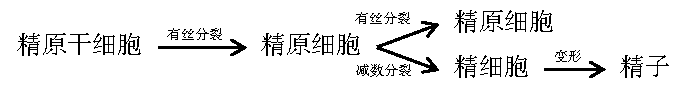
\includegraphics{精子的产生过程}
	\caption{精子的产生过程}
	\label{fig:精子的产生过程}
\end{figure}


\begin{figure}[htbp]
	\centering
	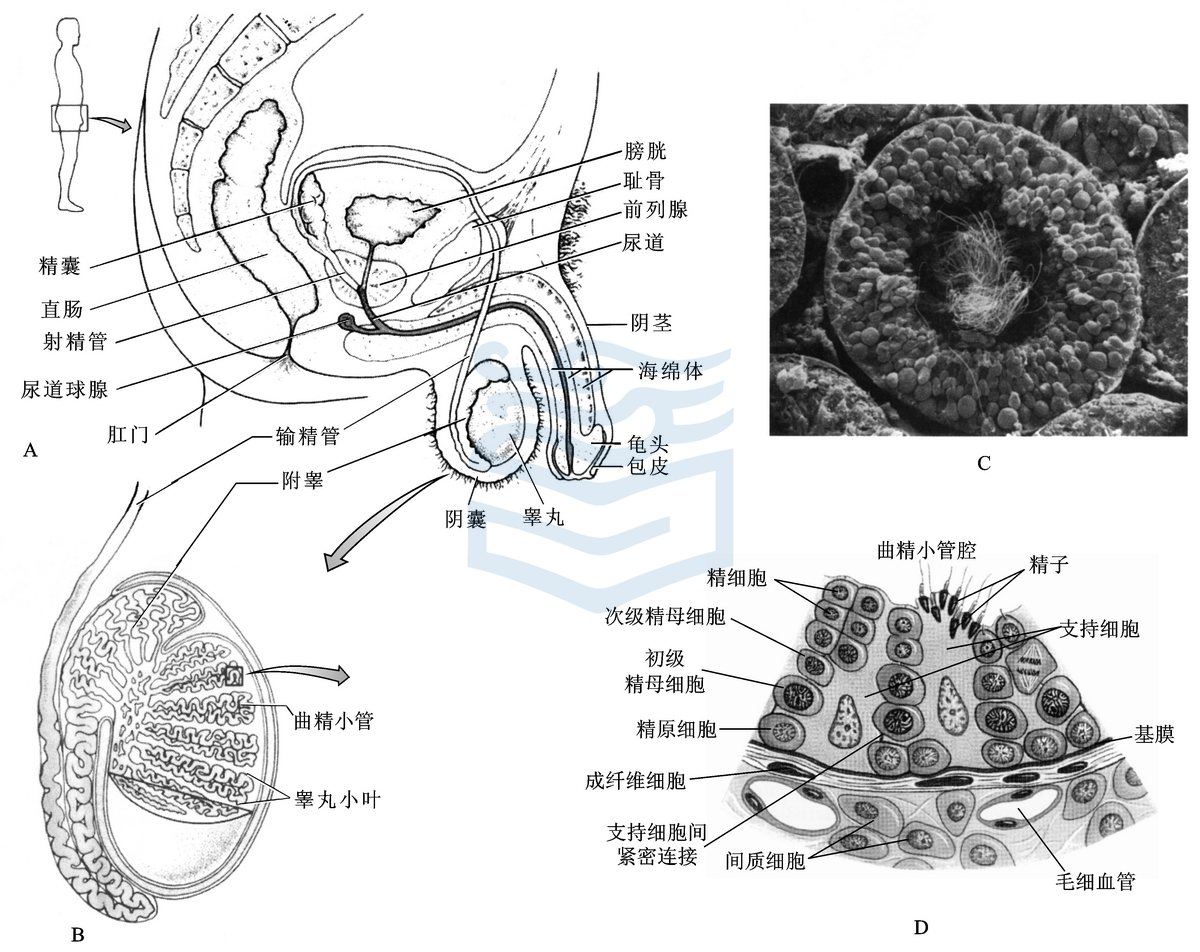
\includegraphics[width=\linewidth]{曲细精管结构示意图.jpg}
	\caption{曲细精管结构示意图}
	\label{fig:曲细精管结构示意图}
\end{figure}

生精过程需要合适的理化环境,若环境不适宜可导致生精障碍:
\begin{itemize}
	\item \sy{隐睾症},即阴囊滞留于腹腔,可导致生精障碍。生精所需温度比体温低,体外的阴囊提供了这一条件;
	\item 局部炎症、酒精中毒、发烧、高温可能导致生精障碍;
	\item 维生素和微量元素缺乏也会导致生精障碍。
\end{itemize}

从睾丸产生的精子,\zhongdian{只有到附睾中停留18\textasciitilde24小时,才获得运动和受精能力。}附睾中同时还存在一些抑制精子活动和受精的物质,使其处于静止状态。

\zhongdian{精液是附睾、前列腺、精囊、尿道球腺的分泌物和精子的混合物。}常通过精液分析来判断男性的生殖能力。

精子在女性体内可存活24\textasciitilde48小时。精子经处理后冷冻可保存很多年。

\subparagraph{支持细胞在生精过程中的作用}

\begin{description}
	\item[支持、保护、营养] 支持细胞伸出突起包围着生精细胞,并形成缝隙连接等细胞连接。支持细胞上有卵泡刺激素(FSH)受体、雄激素受体,受激素调节,调控生精。
	\item[形成血-睾屏障] 支持细胞之间形成紧密连接,可避免生精细胞的抗原物质引发免疫反应。生精细胞向管腔侧的迁移依赖于紧密连接的松解和再组合(磷酸化、去磷酸化)。
	\item[分泌、内分泌] 分泌物有:\begin{itemize}
		\item 雄激素结合蛋白(ABP),转运间质细胞分泌的睾酮至曲细精管,利于生精;
		\item 金属结合蛋白、维生素结合蛋白,转运营养;
		\item 液体,在曲细精管中帮助精子转运;
		\item 芳香化酶,将睾酮转换为雌激素。一定量的雌激素有利于生精;
		\item 抑制素,调控生精。
	\end{itemize}
	\item[吞噬] 吞噬精子细胞变形阶段丢失的胞质、死亡的精子。
\end{description}

\paragraph{睾丸的内分泌功能——产生雄激素}

\sy{睾丸间质细胞}分泌的\sy{雄激素}包括:\zhongdian{脱氢表雄酮(DHEA)、雄烯二酮、睾酮(T)}。睾酮的分泌量和生物活性都是最强的。男性血浆中的睾酮大部分来自睾丸。睾酮从胎儿到出生后6个月由胚胎型间质细胞分泌,青春期之后由成年型间质细胞分泌。

\subparagraph{雄激素的代谢}

\begin{itemize}
	\item 间质细胞主要利用LDL中的胆固醇,少量是HDL。还可通过光面内质网从醋酸盐、乙酰CoA合成胆固醇;
	\item 胆固醇在线粒体中最终生成睾酮。(\autoref{fig:雄激素合成路径})
\end{itemize}

睾酮在血液中多与\sy{性激素结合球蛋白(SHBG)}、血浆白蛋白、皮质醇结合蛋白结合,少数游离。仅游离状态有活性。

睾酮进入靶细胞,可直接发挥作用,也可被5$\upalpha$-还原酶还原为作用更强大的\sy{双氢睾酮}。睾酮在肝脏灭活。

\begin{figure}[htbp]
	\centering
	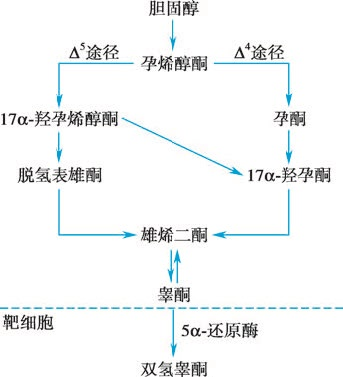
\includegraphics[width=0.5\linewidth]{雄激素合成路径}
	\caption{雄激素合成路径}
	\label{fig:雄激素合成路径}
\end{figure}

\subparagraph{睾酮的生理作用}

\begin{description}
	\item[胚胎性别分化] 促使男性第一性征形成。若男胎胚胎型间质细胞发育不良或对hCG反应低下,导致睾酮分泌不足,最终内外生殖器不能正常分化,形成\sy{假两性畸形}。女胎受过多雄激素作用也可导致假两性畸形。
	\item[促进男性\sy{第二性征}发育] 性器官的发育,胡须、喉结等变化。
	\item[影响生精] 作用于支持细胞,促进生精。
	\item[影响代谢] 多方面的:
	\begin{itemize}
		\item 促进蛋白质合成,抑制蛋白质分解;
		\item 增加血中LDL,减少血中HDL,使男性易患心血管疾病;
		\item 类似肾上腺皮质激素,使钠、水潴留。
	\end{itemize}
	\item[其他作用] \begin{itemize}
		\item 促进肾脏合成EPO,刺激红细胞生成;
		\item 刺激骨生长、骨垢闭合;
		\item 作用于中枢神经系统,调节雄性特征的行为活动。
	\end{itemize}
\end{description}

\subsubsection{睾丸功能的调节}

\paragraph{下丘脑-垂体-睾丸轴的调节}

青春期开始后,下丘脑合成\sy{促性腺激素(GnRH)},脉冲式释放。作用于腺垂体,分泌\sy{卵泡刺激素(FSH)}和\sy{黄体生成素(LH)}。LH的分泌也呈脉冲式,而FSH波动很小。

FSH可:

\begin{itemize}
	\item 作用于支持细胞,促进支持细胞合成生精相关物质,启动生精;
	\item 促进支持细胞合成ABP;
	\item 诱导间质细胞上调LH受体表达,间接促进睾酮分泌。
\end{itemize}

LH作用于间质细胞,促进胆固醇的摄取利用,提高酶活性,促进睾酮生成。

抑制素是一种糖蛋白,可抑制腺垂体FSH的合成和分泌。(\autoref{fig:睾丸的分级调节})

\begin{figure}[htbp]
	\centering
	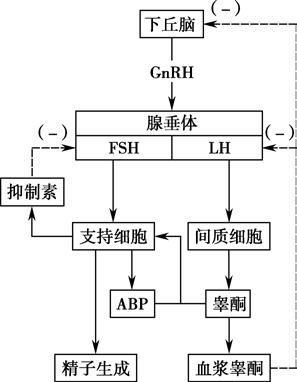
\includegraphics[width=0.3\linewidth]{Pics/睾丸的分级调节}
	\caption{睾丸的分级调节}
	\label{fig:睾丸的分级调节}
\end{figure}


由于睾酮对下丘脑和腺垂体的反馈抑制,对于滥用雄激素导致生精障碍者,应用hCG或芳香化酶抑制剂来治疗,而不是直接给予雄激素。

\paragraph{睾丸内的局部调节}

睾丸内,一些局部调节因子,如生长因子、胰岛素样因子、免疫因子,也以自分泌或旁分泌方式调节睾丸功能。

\subsection{女性生殖功能}

\subsubsection{卵巢的功能}

\paragraph{卵巢的生卵作用}

\subparagraph{卵子的生命历程}

\begin{itemize}
	\item 胚胎时期的原始生殖细胞开始逐渐转化为卵原细胞、初级卵母细胞;
	\item 出生6个月,所有卵母细胞停留在减数第一次分裂前期,细胞核呈泡状,称生发泡;
	\item 青春期后,随卵泡成熟,排卵前在LH峰作用下,继续进行减数分裂,停滞在减数第二次分裂中期。
	\item 若受精,则继续分裂,若没有受精,卵细胞就将死亡。
\end{itemize}

\subparagraph{卵泡的生长发育}

卵泡分为原始卵泡、初级卵泡、次级卵泡、成熟卵泡四类。

\begin{description}
	\item[原始卵泡] 初级卵母细胞+单层梭形颗粒细胞,处于生长静止状态。原始卵泡会逐渐闭锁、退化,从胚胎到性成熟时,数量大减。
	\item[初级卵泡] 卵母细胞略增大,前颗粒细胞发育为多层的立方状颗粒细胞,二者有缝隙连接。透明带形成。卵泡外基质细胞分化为泡膜细胞。
	\item[次级卵泡] 颗粒细胞表达FSH受体、合成芳香化酶,分泌液体形成窦状卵泡。此前的卵泡统称窦前卵泡。

	\hspace{2em} 内泡膜层细胞表达LH受体,参与卵泡激素合成。

	\hspace{2em} 早期窦状卵泡产生抗米勒氏管激素(AMH),抑制原始卵泡的激活。AMH是判断卵泡储备和生殖潜能的重要指标。
	\item[成熟卵泡] 卵丘、放射冠形成。颗粒细胞合成的芳香化酶活性增加,合成雌激素也最多。
\end{description}

卵泡发育分为三个阶段:

\begin{description}
	\item[FSH非依赖的缓慢生长] 卵泡生长完全不依赖促性腺激素,非常缓慢。从胎儿到绝经前均可发动这一时期的卵泡生长。
	\item[FSH反应性生长] 青春期后FSH分泌,陆续有卵泡对FSH做出反应,加快生长速度。
	\item[FSH高度依赖的快速生长] 月经周期中黄体期向卵泡期转化时,垂体FSH分泌增加,卵泡周期性募集。仅有一个卵泡会成为优势卵泡,最终发育成熟。这就是优势卵泡的选择。
\end{description}

卵泡选择机制,目前公认的是FSH阈值学说。

\begin{itemize}
	\item FSH阈值是卵泡生长发育所需的最小FSH浓度,反映卵泡对FSH的敏感性。
	\item 卵泡期刚开始时,FSH浓度足够所有被募集的卵泡发育。
	\item 随着卵泡生长,雌激素分泌增加、颗粒细胞产生的抑制素二者都使FSH浓度降低。
	\item 此时,FSH浓度只能满足阈值最低的那个卵泡发育成熟。
	\item 选择的过程一般发生在月经周期的5\textasciitilde7天。
\end{itemize}

FSH浓度高,卵泡募集$\longrightarrow$卵泡产生雌激素,使FSH降低$\longrightarrow$只有阈值较低的卵泡才能发育。

甾体类口服避孕药就是通过外源雌激素、孕激素,抑制FSH分泌,干扰卵泡选择,从而避孕。

\subparagraph{排卵}

LH峰触发排卵,成熟卵泡的卵泡壁破裂,卵母细胞和放射冠一起排出卵泡。

\subparagraph{黄体的形成和退化}

排卵后,剩余的颗粒细胞和泡膜细胞在LH作用下,形成黄体。

黄体的主要功能是分泌孕激素、雌激素,促使子宫内膜形态变化,以适应早期胚胎发育及着床需要。

\begin{itemize}
	\item 若卵受精,则黄体在胚胎滋养层分泌的hCG作用下发育为妊娠黄体,怀孕3个月后由胎盘接替黄体的内分泌功能。
	\item 若未受精,2周后黄体开始退化,最后成为白体,是结缔组织瘢痕。
\end{itemize}

\subparagraph{卵泡闭锁}

卵泡闭锁指的是卵泡在发育过程中退化,是细胞凋亡所致。

\paragraph{卵巢的内分泌功能}

排卵前的卵泡主要分泌雌激素,包括雌酮、雌二醇(E$_{2}$),二者可互变,雌二醇的活性最强。

排卵后的黄体分泌雌激素和孕激素。孕激素主要是孕酮。

卵巢也合成分泌少量雄激素和抑制素。

\subparagraph{卵巢性激素的代谢}

卵泡雌激素合成由内泡膜细胞和颗粒细胞共同完成。(\autoref{fig:雌激素的合成})

\begin{figure}[htbp]
	\centering
	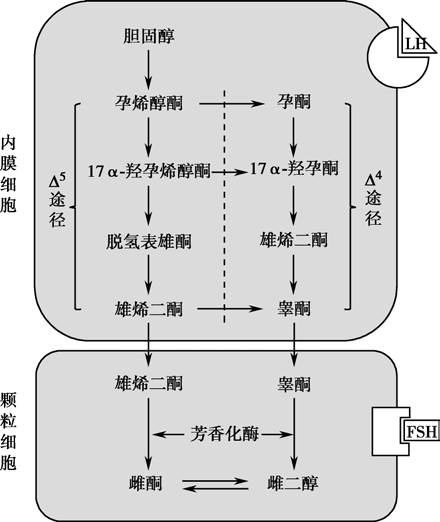
\includegraphics[width=0.5\linewidth]{Pics/雌激素的合成}
	\caption{雌激素的合成}
	\label{fig:雌激素的合成}
\end{figure}

\begin{itemize}
	\item 内泡膜细胞在LH作用下,以胆固醇为原料合成雄烯二酮和睾酮,这一步在任意阶段的卵泡中均能进行。
	\item 发育到一定阶段的卵泡中,颗粒细胞在FSH作用下产生芳香化酶,将雄激素转变为雌激素。随着卵泡生长,合成的雌激素增多,雄激素减少。
\end{itemize}

血中雌激素和孕激素也主要通过与SHBP、白蛋白结合运输,仅游离状态的有活性。

\subparagraph{雌激素和孕激素的作用}

雌激素、孕激素都是既可“慢反应”,也可“快反应”。雌激素和孕激素的作用有时协同,有时拮抗。

\begin{table}[htbp]
	\centering
	\begin{tabularx}{\textwidth}{|c|X|X|}
		\hline
		部位 & \multicolumn{1}{c|}{雌激素的作用} & \multicolumn{1}{c|}{孕激素的作用} \\ \hline
		子宫肌 & 促细胞增生肥大,增强对收缩刺激的反应性 & 降低孕期子宫对收缩刺激的反应 \\ \hline
		子宫内膜 & 促内膜细胞增殖、腺体增生 & 促内膜上皮分泌及基质细胞蜕膜化 \\ \hline
		宫颈 & 排卵期松弛,分泌清而稀薄的黏液 & 黏液分泌减少、黏稠 \\ \hline
		输卵管 & 促进纤毛摆动,增强收缩性 & 促进分泌,抑制收缩性 \\ \hline
		阴道 & 促进上皮细胞增殖,角化,维持酸性环境 & 抑制上皮细胞增殖,加快脱落 \\ \hline
		乳腺 & 促进乳腺导管发育,脂肪聚集 & 促进乳腺小叶及腺泡发育 \\ \hline
		下丘脑、垂体 & 卵泡期负反馈,月经中期正反馈 & 黄体期负反馈,兴奋下丘脑体温调节中枢 \\ \hline
		代谢 & 水钠潴留,有利骨质代谢、脂代谢 & 促水钠排出 \\ \hline
	\end{tabularx}
	\caption{雌激素和孕激素的作用}
	\label{tab:my-table}
\end{table}

\subsubsection{月经周期}

月经周期平均28天,具体长度因人而异。

\paragraph{月经周期的分期}

见\autoref{tab:月经周期的分期}。

\begin{table}[htbp]
	\centering
	\begin{tabularx}{\textwidth}{|c|c|c|C|}
		\hline
		\textbf{分期} & 卵泡期(增生期) & 黄体期(分泌期) & 月经期 \\ \hline
		\textbf{时间} & 第1\textasciitilde14天 & 第15\textasciitilde28天 & 第1\textasciitilde5天 \\ \hline
		\textbf{卵泡} & 快速生长 & 排卵后形成黄体 & 卵未受精,黄体萎缩退化 \\ \hline
		\textbf{子宫内膜} & 开始修复 & 蜕膜化改变 & 脱落出血 \\ \hline
		\textbf{雌激素} & 增加 & 大量 & 突降 \\ \hline
		\textbf{孕激素} & --- & 大量 & 突降 \\ \hline
		\textbf{宫颈粘液} & 稀薄、透明 & 粘稠、浑浊 & --- \\ \hline
	\end{tabularx}
	\caption{月经周期的分期}
	\label{tab:月经周期的分期}
\end{table}

月经周期的第20\textasciitilde23天为着床窗口期。

月经周期中黄体期时长相对稳定,卵泡期长度变化较大,故临床上将月经来潮前的前14天作为排卵日。

\paragraph{月经周期的调控}

\subparagraph{下丘脑-垂体-卵巢轴的功能}

青春期后,下丘脑GnRH神经元成熟,脉冲式释放GnRH,促使腺垂体分泌FSH和LH。详见\autoref{fig:卵巢的分级调节}。GnRH神经元受神经递质kisspeptin的调控。

\begin{figure}[htbp]
	\centering
	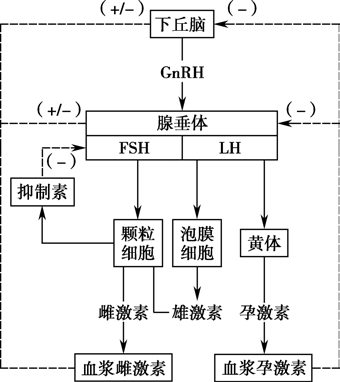
\includegraphics[width=0.3\linewidth]{Pics/卵巢的分级调节}
	\caption{卵巢的分级调节}
	\label{fig:卵巢的分级调节}
\end{figure}

\subparagraph{月经周期各期的内分泌调控}

\begin{description}
	\item[卵泡期早期] 前次月经周期的黄体退化,孕激素和雌激素减少,反馈抑制解除,FSH和LH增加。随后发生卵泡募集,雌激素增加,FSH降低。
	\item[月经周期中期] 优势卵泡成熟,雌激素水平进一步增加,正反馈下丘脑和垂体,GnRH、LH、FSH大量释放,出现LH峰。
	\item[黄体期] 雌激素分泌因排卵而下降,后在LH作用下黄体发育,孕激素和雌激素都升高。而FSH和LH受负反馈,含量较低。若未受精,则黄体退化后雌激素、孕激素减少,FSH、LH增加。由此进入下一个月经周期。
\end{description}

月经周期中激素、卵泡及子宫内膜的变化如\autoref{fig:月经周期中生殖激素、卵巢和子宫内膜的变化}。

\begin{figure}[htbp]
	\centering
	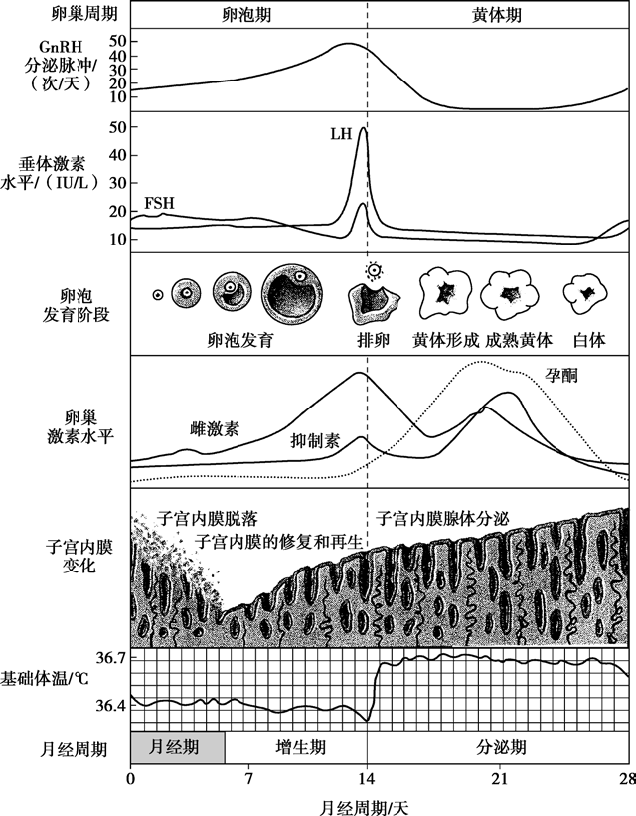
\includegraphics[width=0.7\linewidth]{Pics/月经周期中生殖激素、卵巢和子宫内膜的变化}
	\caption{月经周期中生殖激素、卵巢和子宫内膜的变化}
	\label{fig:月经周期中生殖激素、卵巢和子宫内膜的变化}
\end{figure}

\subparagraph{其他激素对月经周期的影响}

如催乳素(PRL)、甲状腺素和胰岛素都参与卵巢的调控。

\subsubsection{卵巢功能的衰退}

从卵巢功能开始衰退到完全丧失后一年的时间称为围绝经期(更年期)。卵巢对FSH和LH的反应性下降,卵泡发育停滞不能排卵。卵巢功能进一步衰退,卵泡几乎完全耗尽,则进入绝经期。

处于围绝经期的妇女因雌激素分泌水平下降,可能出现围绝经期综合征。

\subsection[妊娠]{\xpinyin*{妊娠}}

妊娠包括受精、着床、妊娠维持、分娩。若从最后一次月经的第一天开始算,人类的妊娠时间为280天。

\subsubsection{受精}

\paragraph{精子运动}

精子需要经过子宫颈、子宫腔、输卵管到达输卵管壶腹受精。

有利于精子在女性生殖道内运动的因素:
\begin{itemize}
	\item 宫颈分泌的粘液透明清亮,利于精子穿行。
	\item 雌激素还可刺激输卵管蠕动,推动精子。
	\item 精液中的前列腺素可使子宫收缩,把精子吸入。
\end{itemize}

排卵后孕激素使宫颈粘液变得粘稠、浑浊,可阻碍精子运动。

\paragraph{精子获能}

精子在女性生殖道停留,发生形态和功能变化,获得受精的能力,成为精子获能。

\paragraph{顶体反应}

精子头部的顶体外膜破裂,释放出酶溶解卵细胞外围的透明带和放射冠。(\autoref{fig:精卵相互作用的示意图})

\begin{figure}[htbp]
	\centering
	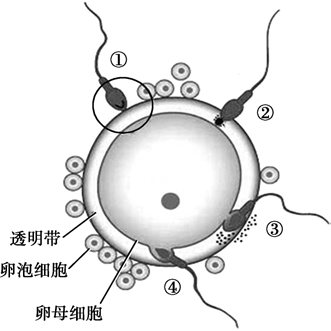
\includegraphics[width=0.3\linewidth]{Pics/精卵相互作用的示意图}
	\caption{精卵相互作用的示意图}
	\label{fig:精卵相互作用的示意图}
\end{figure}


\paragraph{受精卵形成}

主要包括下列变化:

\begin{itemize}
	\item 精子与卵细胞融合后,卵内$[\ce{Ca^{2+}}]$升高,透明带变硬;
	\item $[\ce{Ca^{2+}}]$升高,使卵激活,完成第二次减数分裂,形成合子。
\end{itemize}

\subsubsection{着床}

成功的着床需要胚泡发育和子宫内膜蜕膜化彼此同步。卵巢雌激素和孕酮诱导蜕膜化。

胚泡的植入是同种异体植入过程。胚泡分泌hCG来抑制母体的免疫反应。

\subsubsection{妊娠的维持}

妊娠10周内,由妊娠黄体承担内分泌功能。之后胎盘形成,妊娠黄体退化,接替其内分泌功能。胎盘的形成才使妊娠得以维持。

\paragraph{胎盘}

\subparagraph{胎盘的物质转运功能}

胎盘血液与母体并不相通,通过胎盘屏障将二者隔开。母体和胎儿之间,\ce{CO2}和\ce{O2}以简单扩散、葡萄糖和氨基酸以主动运输、脂肪酸以简单扩散进行交换。

\subparagraph{胎盘的内分泌功能}

\begin{description}
	\item[人绒毛膜促性腺激素(hCG)] 早起胚泡和合体滋养层分泌的糖蛋白。促进胚泡植入、妊娠黄体的形成,维持妊娠。早期妊娠可用hCG的存在来确定。
	\item[人胎盘生乳素(hPL)] 又称人绒毛膜促生长激素(hCS),因为它和生乳没有任何关系,主要是促进胎儿生长。
	\item[雌激素] 胎盘分泌的雌激素主要是雌三醇。雌三醇的形成涉及胎盘和胎儿的共同参与。
	\item[孕激素] 胎盘产生孕酮,维持妊娠期子宫处于静息状态。
\end{description}

\paragraph{母体的适应性变化}

\begin{description}
	\item[心血管系统] 妊娠期母体的血容量和心输出量增大,但血压不升高;
	\item[内分泌] 垂体、肾上腺、甲状腺、甲状旁腺的活动增强。甲状旁腺活动增强可使血中游离\ce{Ca^{2+}}升高,满足胎儿骨骼生长需要。
	\item[呼吸] 肺通气增强,因子宫对膈肌的压迫和孕激素对呼吸中枢的作用。
	\item[泌尿] 肾脏稍增大,因血容量增加导致肾脏负荷增加所致。
	\item[能量代谢] 妊娠前期不怎么变化。从妊娠中期开始,母体的基础代谢率逐渐升高。
\end{description}

\subsubsection{分娩}

分娩是正反馈的过程。一旦子宫开始阵发性收缩,腹壁肌肉和膈肌也会收缩。子宫是阵发性收缩而不是强直性收缩,意义是防止胎儿窒息。

分娩启动的机制尚不完全清楚。分娩启动需要胎儿、胎盘、母体因素的共同作用。包括:
\begin{itemize}
	\item 胎儿对子宫的机械性扩张;
	\item 胎儿自己的肾上腺皮质分泌糖皮质激素,促使胎盘的孕激素向雌激素转化,提高雌激素水平。
	\item 前列腺素在分娩发动中起重要作用。
	\item 缩宫素是母体来源的、在分娩过程中起重要作用的激素。但它不是分娩发动的决定因素。
\end{itemize}